%% THIS IS THE MAIN FILE %%
% Here the main arrangement of your thesis is determined. 
% In this file you read in all chapters (as separate .tex files)
% This is also the file you 'Build' with a LaTeX editor, like TeXmaker.
% The .cls file (mscThesis.cls) contains all details regarding copyrights and so on. Take a look and adjust where applicable.
% This MSc thesis standard layout is optimized for double sided printing on A4 format paper.
% Good luck and have fun with your Master Research in Applied Geophysics! Kind regards, Niels Grobbe
\documentclass[a4paper,11pt]{mscThesis}
%
%\usepackage{pifont}
\usepackage{amssymb}
\usepackage{amsmath}
\usepackage{subcaption}
\usepackage{placeins}
\usepackage{natbib}
\usepackage{siunitx}
%\usetikzlibrary{matrix}
\usepackage{todonotes}
\usepackage{caption}
\usepackage{subcaption}
\usepackage{verbatim}

\mscName{Christian Reinicke Urruticoechea}
\mscDate{\today}
\mscTitle{Seismic deblending of simultaneous crossline sources}
\mscSubTitle{}
\mscKeyWords{thesis, msc, subject}
%
%\mscBackPicture{2660PF3}    % eps of 21 * 29.7 cm
\mscReaderOne{Dr. Ir. G.J.A. van Groenestijn}
\mscReaderTwo{Dr. Ir. G.G.Drijkoningen}
\mscReaderThree{Dr. Christoph Clauser}
%\mscReaderFour{}
%
\setThesisInfo
%
\begin{document}
%
%============================= Front matter ========================================
\frontmatter %
%
% Make a hell of a lot of title pages
    \maketitle
%
% Abstract
    \nonumchap{Abstract}

    This is the shortest abstract you have ever seen.
    \cleardoublepage
%
% Acknowledgements
    \nonumchap{Acknowledgements}%
    First of all I want to thank all the people who have participated in this project ..
    Remember, often more people have contributed to your final thesis than you initially would think of.
    \vspace*{15mm}

    \noindent
    Delft, University of Technology \hfill \mscname\\ % change to the university where you carried out your final MSc thesis research
    \mscdate

%
% table of contents, (\toc of \toclof of \tocloflot )
    \tocloflot
%
% Nomenclature
    \printnomencl %
%
% Acronyms
    \nonumchap{Acronyms} %
    %
    \begin{acronym}%
        \acro{DUT}{Delft University of Technology}%
    \end{acronym}%
    %
    \cleardoublepage%
%
%
%============================= Main matter =========================================
%
\mainmatter
%
% Introduction
\chapter{Introduction} \label{chap::intro}

    Welcome to the standard layout for your IDEA LEAGUE MSc thesis written in \LaTeX. \LaTeX\  has a variety of advantages over conventional/ standard text editing programs, which you will soon enough discover yourself. \LaTeX\  almost forms a standard in the Scientific Community, especially due to its effective and straightforward mathematical capabilities.\\
    This is Chapter\ \ref{chap::intro}. If you want to know more about \LaTeX\ you better read
    \cite{texbook} or use the extensive help available on the internet. \index{LaTeX}. This 'hidden' index command helps you making an index at the end of your thesis. You can add this flag anywhere you want to make an index hit. You can see here also how to use acronyms, like \ac{DUT}. The acronyms are automatically listed in the corresponding section. Also, hyperlinks are created automatically with the developed class file, such that your digital PDF version of your thesis can be read dynamically.
 Have fun with \LaTeX\ and your M.Sc. research project and good luck! \\ \\
 
The purpose of the introduction is to tell readers why they should want to read what follows the introduction. This chapter should provide sufficient background information to allow readers to understand the context and significance of the problem. This does not mean, however, that authors should use the introduction to rederive established results or to indulge in other needless repetition. The introduction should (1) present the nature and scope of the problem; (2) review the pertinent literature, within reason; (3) state the objectives; (4) describe the method of investigation; and (5) describe the principal results of the investigation. % notice how the reference to the introduction takes place.. It refers to the name.tex
\cleardoublepage

%
% First Part
    %\part{First Part} % you can divide your thesis into different parts, for example Theory&Modeling in part 1 and real data examples in part 2.
		%    \chapter{First Real Chapter}

    This is a demonstration chapter. I will explain some of the possibilities of \LaTeX. Here something will be shown of control theory, 'the transfer function' \lsymb{$H(s)$}{Transfer function}. Subscripts and superscripts can be put in the nomenclature \index{nomenclature} list. \supers{max}{Maximum} \subs{min}{Minimum} Other things can also be added to the nomenclature list, like explanations of symbols being used throughout the thesis. \others{[kts]}{Knots} \others{$^{\circ}$, [deg]}{Degrees}

        \section{First section}

        This is the section. Referring to equations, figures and tables can easily be done by the commands \verb"\eqnref{}",
        \verb"\figref{}" and \verb"\tabref{}".
        \begin{equation}\label{eq:First}
        H(s) = \frac{1}{s+2}
        \end{equation}

        You see? Refer to equations like this \eqnref{eq:First}, i.e. the name of the label you have given the specific equation, figure or table.
        
        \subsection{The first subsection}
  
        Now I demonstrate, numbering equations, using subequations:
	  \begin{subequations}
		\begin{eqnarray}
    \label{2eq1d1}
	  \nabla\times\mathbf{L}  &=& \frac{\partial\mathbf{G}}{\partial t} \\
    \label{2eq1d2}
  	\nabla\times\mathbf{G}  &=& \frac{\partial\mathbf{L}}{\partial t} + \mathbf{J} \\
    \label{2eq1d3}
    \mathbf{G}              &=& \sigma\mathbf{J}
		\end{eqnarray}
			  \end{subequations}
	
				Or we can make matrices:
				\begin{equation}
				\mathbf{Q}_{12}=\left[\begin{array}{ccc}
		          0  &     1          &  0 \\
	            1  &     0          &  1 \\
	            0  &     1          &  0 \\
       	\end{array}\right]\quad
        \nonumber
		    \label{2eq1cf}
		    \end{equation}
		    This can also be done using the \verb"\align{}" command. Equation arrays are also possible:
     		\begin{eqnarray}
    		\label{2eq1e1}
	  \nabla\times\mathbf{L}  &=& \frac{\partial\mathbf{G}}{\partial t} \\
	    	\label{2eq1e2}
  	\nabla\times\mathbf{G}  &=& \frac{\partial\mathbf{L}}{\partial t} + \mathbf{J} \\
		    \label{2eq1e3}
    \mathbf{G}              &=& \sigma\mathbf{J}
		  \end{eqnarray}

       
        \subsubsection[Subsection Short Title]{The first sub-subsection with a very very very long title, but in the table of contents one can only see the short title in square brackets}

                Impressed by the capabilities? \index{Nicecapabilities}
                If you want to know more about the capabilities of \LaTeX, take a look at the "\textbf{The Not So Short Introduction to \LaTeXe}", which can be found on the internet.

    \paragraph{Next paragraph.}
    \begin{figure}[htbp]  % fig 6.3 page 186 Turbulence and Remous
    \centering
    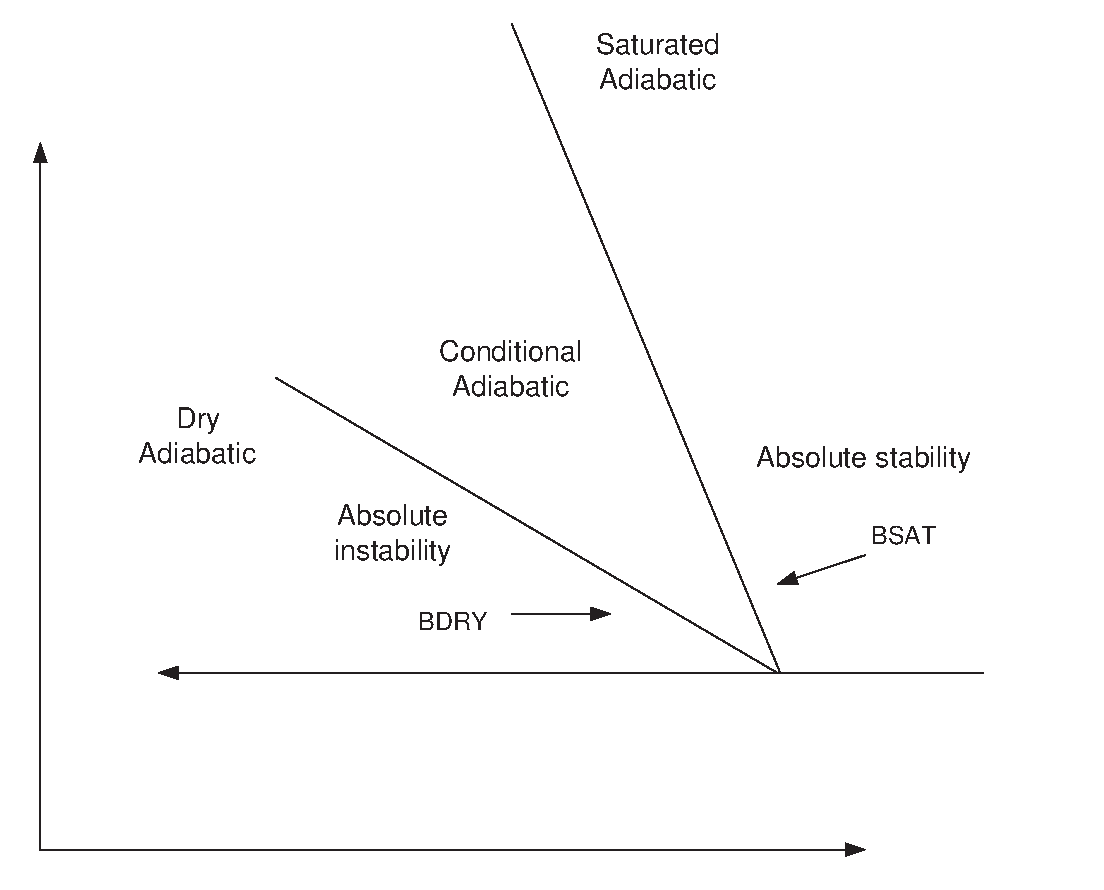
\includegraphics[width=11cm]{vertstab.eps}
    \caption{Stability conditions for the vertical stability of saturated and unsaturated air.} %this is how it shows up in the List of Figures
    \label{f:verticalstab}
    \end{figure}
.\\    
And finally I end this example file with a table which will be centered in the middle of the following page
\begin{table}[hp]
\centering
\renewcommand{\arraystretch}{1.5}
\begin{tabular}{|ll|}
\hline
\multicolumn{2}{|c|}{\bf\sffamily {\it Data} files listed in a table }\\
\hline\hline
\multicolumn{2}{|l|}{\bf\sffamily First part} \\
Fabracadabra.m	& - Saturation computation\\
Fobracadabra.m	& - Pressure computation\\
Fibricadibri.m	& - Permeability computation\\
&\\
\multicolumn{2}{|l|}{\bf\sffamily Structural rock model} \\
struct.m	& - Rock structural data using symmetric boundary condition \\
bstruct.m	& - Rock structural data using anti-symmetric boundary condition \\
\hline
\end{tabular}
\caption{Good-looking program data deck files.} %this is how it shows up in the List of Tables
\label{tbl:tbl}
\end{table}

		
% My part
    \part{Theory}
    	\chapter{Theory} \label{chap:theory}

This chapter describes the theory behind blending and deblending. First the detail hiding operator notation is explained. This notation is used to describe the forward model of seismic data. By introducing the blending operator the forward model is extended to the blended case. Next, the deblending method presented in \citet{Mahdad-Deblending-Method} is discussed to illustrate some of the concepts used in this thesis.

\section{The Forward Model of Blending} \label{sec:Ch-Theory-Operator}
%The detail hiding operator notation was introduced by \citet{Berkhout1982}, and later on it was extended for blended data. 

\subsection{Conventional Seismic Data}
In the detail hiding operator notation \citep{Berkhout1982} the recorded signal is considered discrete in terms of time $t$, receiver position $x_r$, and source position $x_s$. Thus, the measurements can be organized in a cube, $\mathbf{p(t,x_r,x_s)}$ (see Figure \ref{fig:Ch-Theory-DataMatrix}). Each frequency slice of this new cube represents the data matrix, $\mathbf{P}$. 

In the data matrix, $\mathbf{P}$, each column corresponds to a monochromatic common shot gather (see Figure \ref{fig:Ch-Theory-DataMatrixMahdad}), each row to a monochromatic common receiver gather, each diagonal to a monochromatic common offset gather, and each anti-diagonal to a monochromatic common midpoint gather. 

\begin{figure}
    \centering
	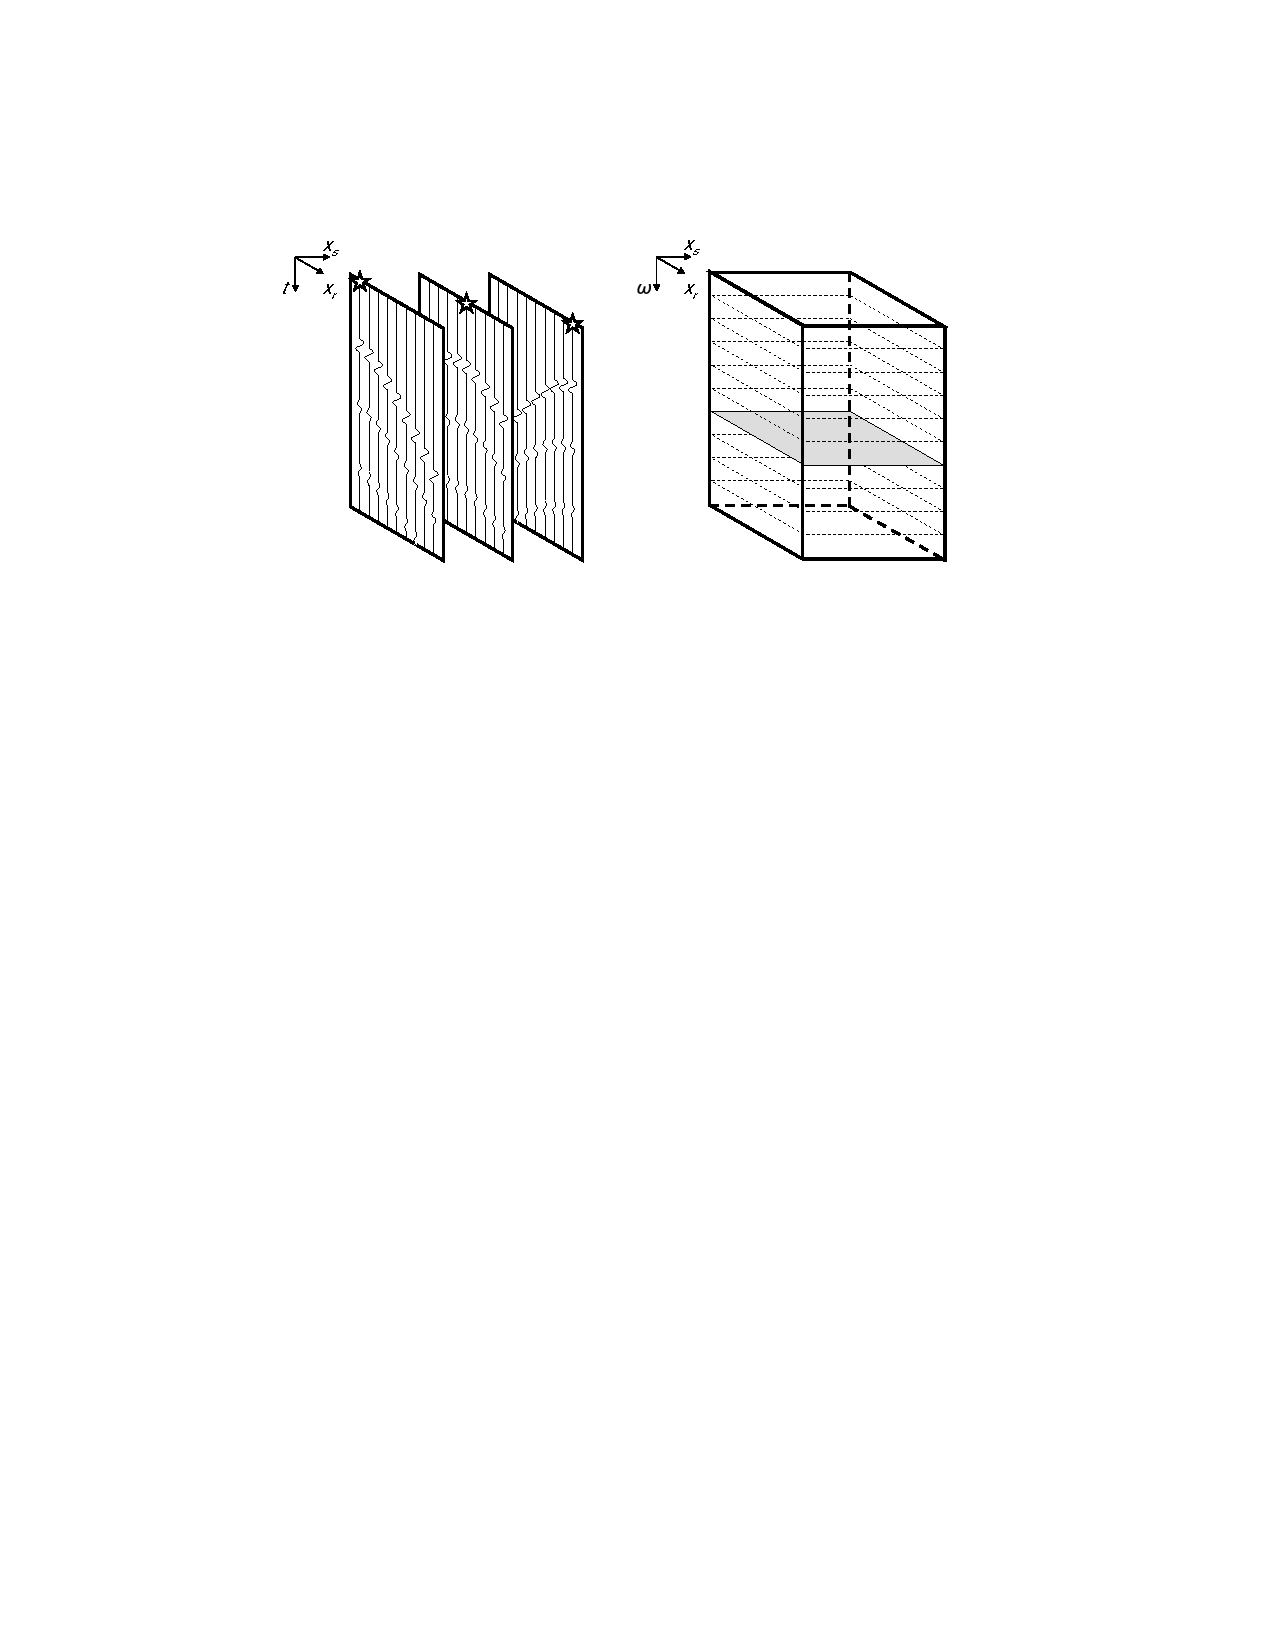
\includegraphics{Plots/P-Groenestijn_2010}
	\caption{Illustration of the data matrix, $\mathbf{P}$, by \citet{Groenestijn_2010}. \textit{Left:} The signal generated at the source position, $x_s$, is measured at receiver position, $x_r$, as a function of time, $t$. Thus, the discretized data is saved in a cube, $\mathbf{p(t,x_r,x_s)}$. \textit{Right:} The cube on the right equals the left cube after a Fourier transform with respect to time. Each frequency slice of the right cube represents the data matrix, $\mathbf{P}$.}
	\label{fig:Ch-Theory-DataMatrix}
\end{figure}


\begin{figure}
    \centering
	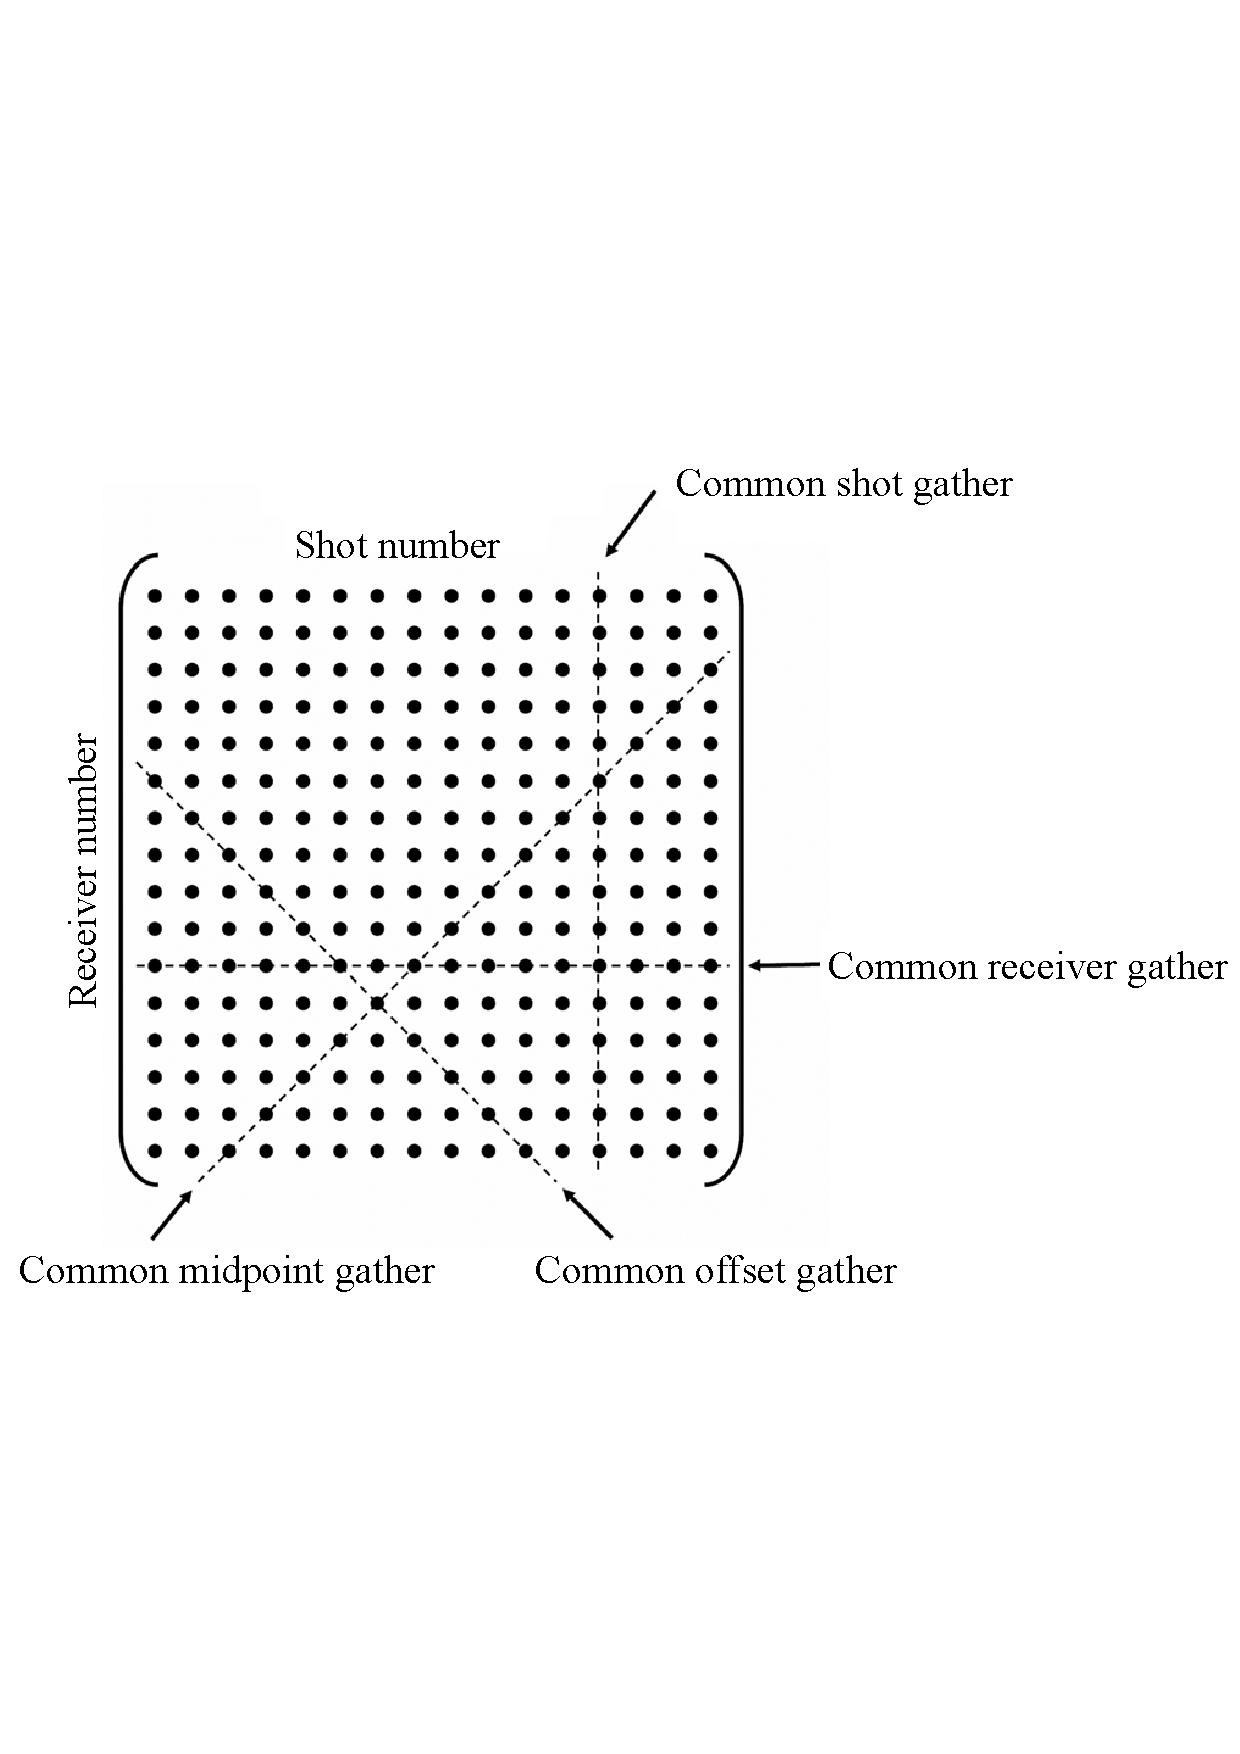
\includegraphics[width = 0.6\textwidth]{Plots/Mahdad-Data-Matrix-edited}
	\caption{Illustration of the data matrix, $\mathbf{P}$, by \cite{Mahdad-Deblending-Method}. The dotted lines indicate directions of common gathers.}
	\label{fig:Ch-Theory-DataMatrixMahdad}
\end{figure}

According to the seismic forward model of \citet{Berkhout1982} the data matrix, $\mathbf{P}$, can be represented by a matrix multiplication of the source matrix, $\mathbf{S}$, the impulse response of the earth, $\mathbf{X}$, and the receiver matrix, $\mathbf{D}$:

\begin{equation}
	\mathbf{P} = \mathbf{D \, X \, S}.
	\label{eq:Ch-Theory-DataRepresentation}
\end{equation}

In the source matrix, $\mathbf{S}$, each row and each column represent one source position (see Figure \ref{fig:Ch-Theory-BlendedSource-Matrices}). Thus, $\mathbf{S}$ is a diagonal matrix. Each diagonal element $s_{ii}$ captures one frequency component of the source signature injected in the earth at the position $x_s = x_i$. By applying a Fourier transform to all frequency components of the element $s_{ii}$ the source signature is obtained.

 The impulse response of the earth, $\mathbf{X}$, describes how an impulse at the source location, $x_s$, is transformed in the earth into the signal at the receiver location, $x_r$.

$\mathbf{D}$ is the receiver matrix, which converts the seismic wavefield at the receiver location $x_r$ to the recorded signal. This includes the forward model of the receiver ghost.

In practice, one tries to retrieve the unknown earth response, $\mathbf{X}$, from the data, $\mathbf{P}$, by removing $\mathbf{S}$ (designature) and $\mathbf{D}$ (receiver deghosting).



\subsection{Blended Seismic Data}

\begin{figure}
	
	\centering
	\begin{subfigure}[t]{0.6\textwidth}	
	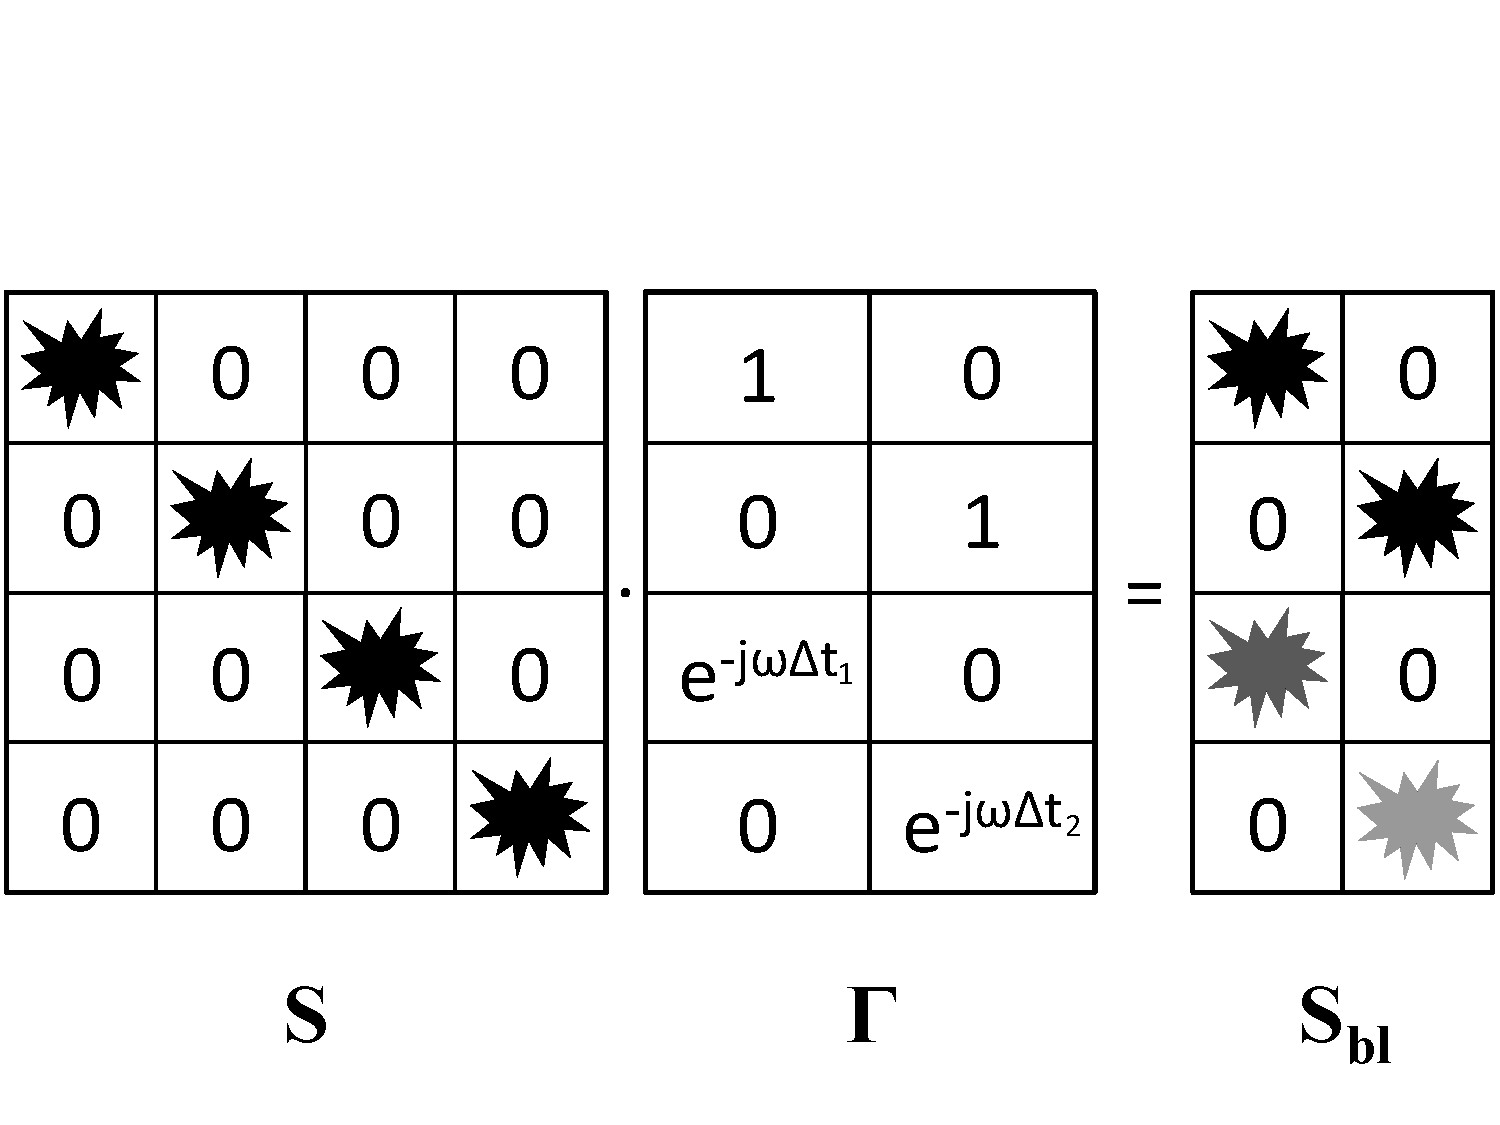
\includegraphics[width=\textwidth]{Plots/Blended-Source-edit2}
	\caption{}
	\label{fig:Ch-Theory-BlendedSource-Matrices}
	\end{subfigure}
	\par\bigskip
	\begin{subfigure}[t]{\textwidth}
	\centering
	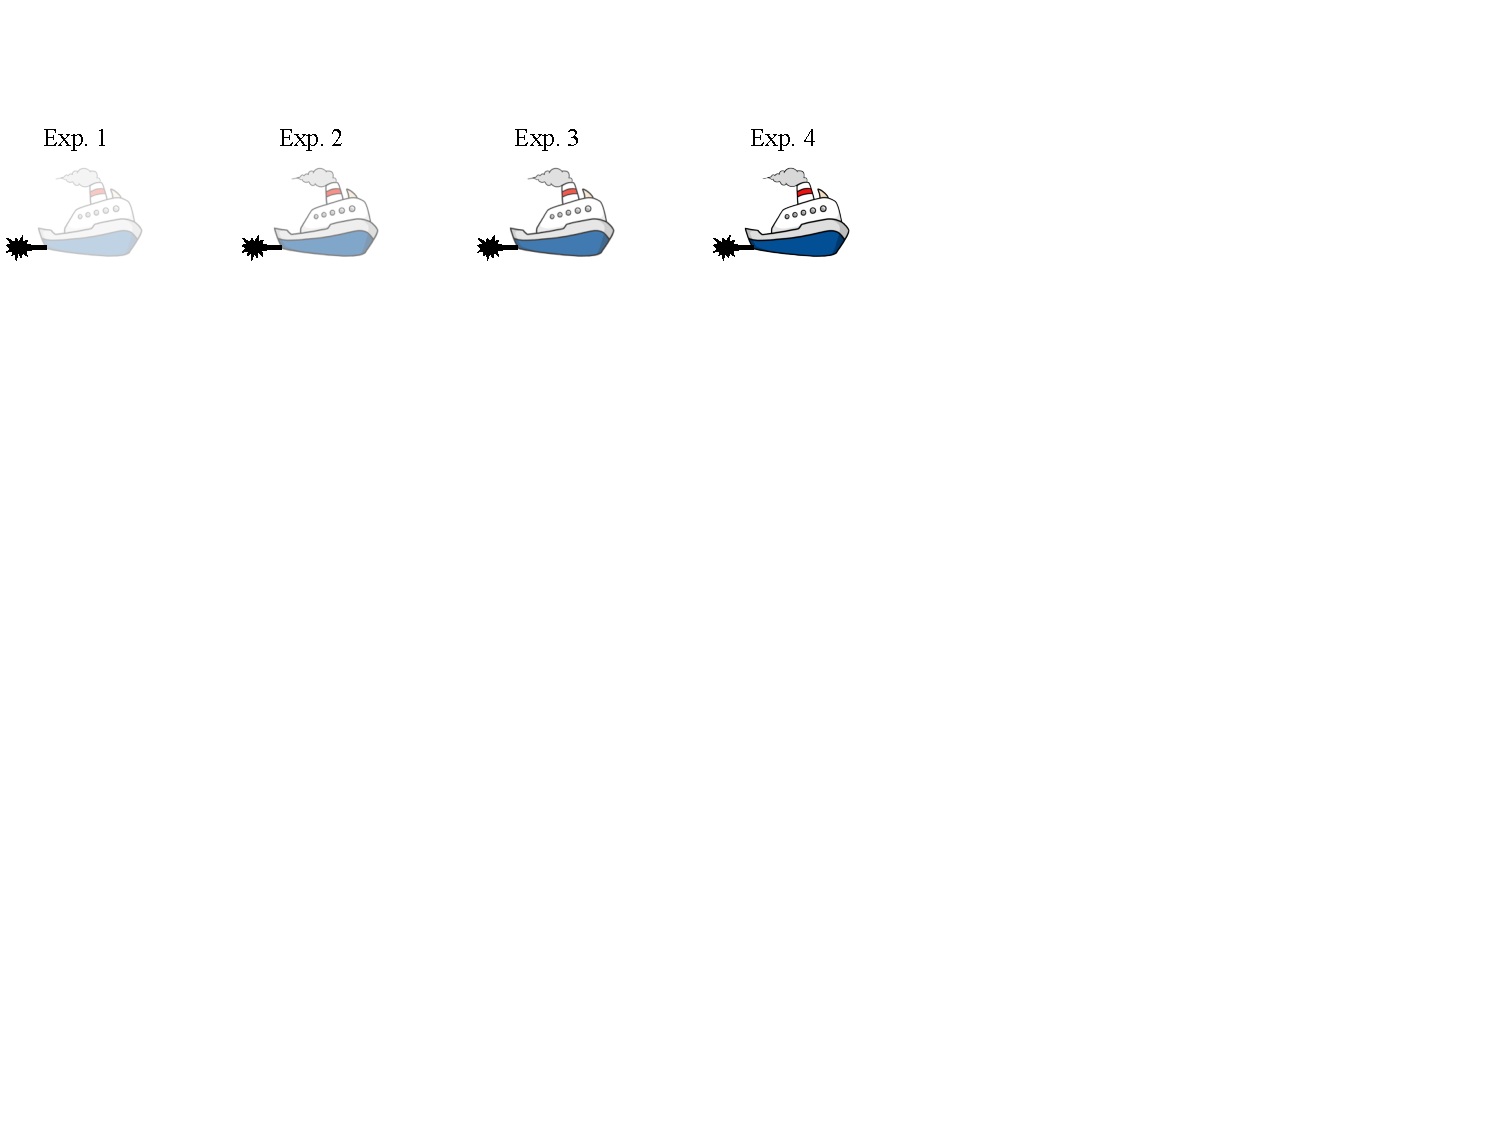
\includegraphics[width=0.5\textwidth]{Plots/Blended-Source-Conventional}
	\caption{}
	\label{fig:Ch-Theory-BlendedSource-Conventional}
	\end{subfigure}
	\par\bigskip
	\begin{subfigure}[t]{\textwidth}
	\centering
	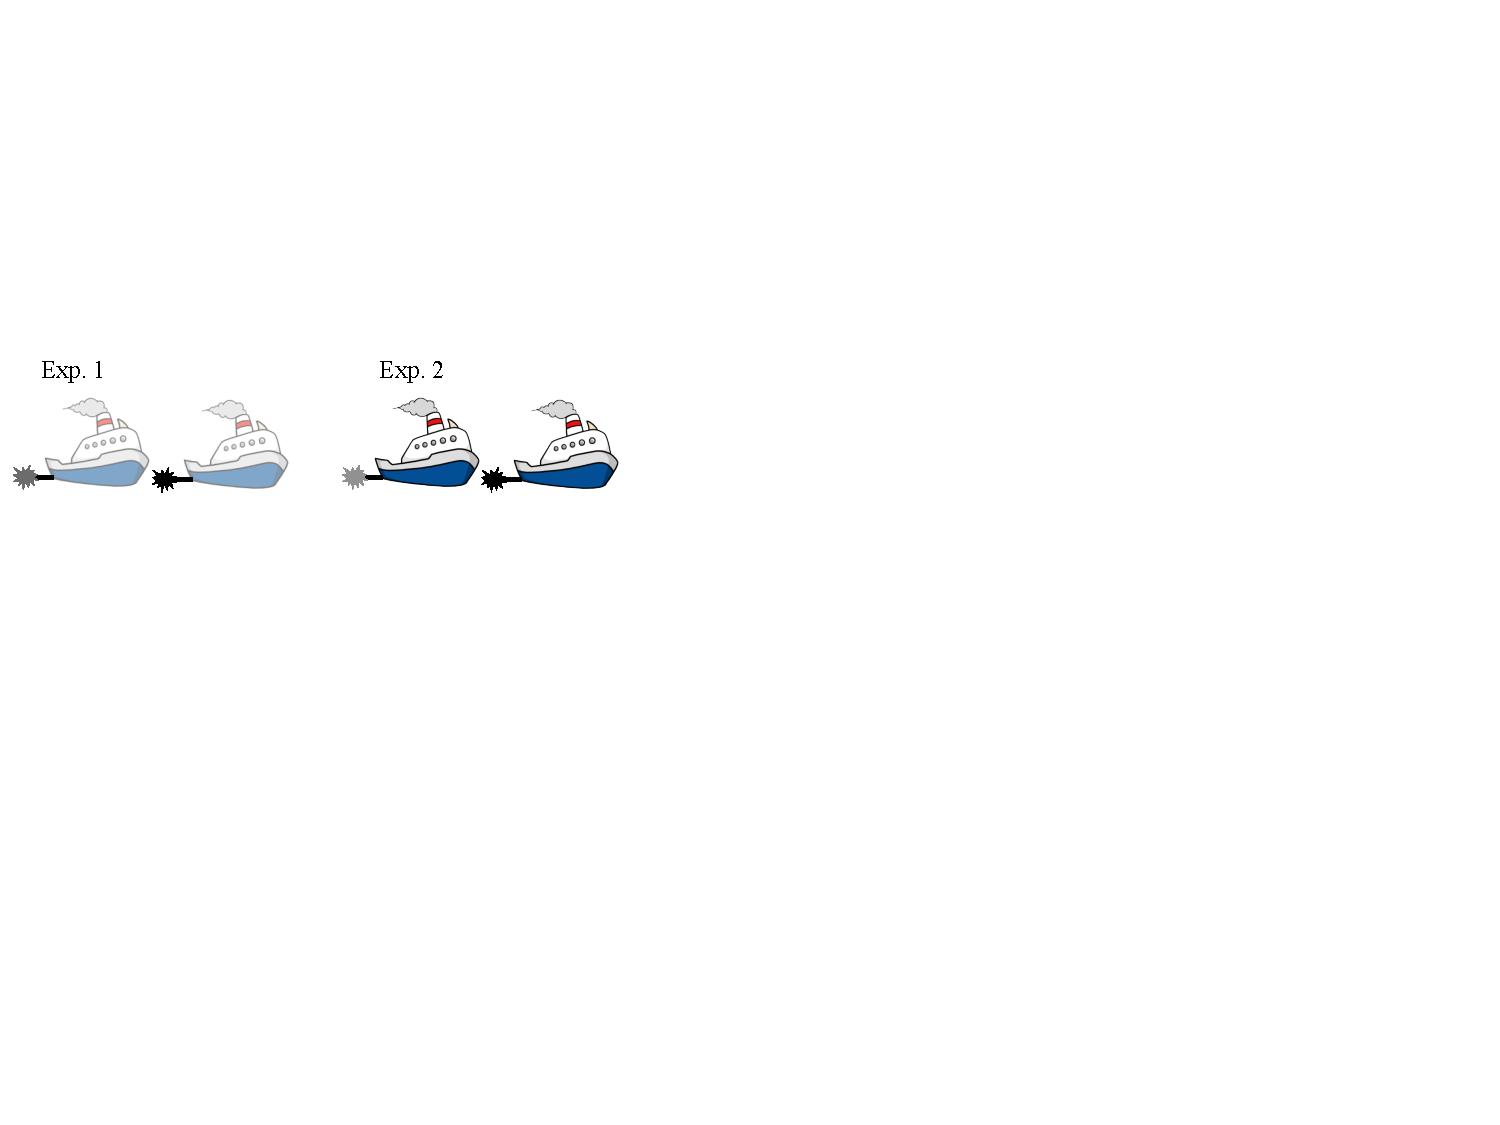
\includegraphics[width=0.36\textwidth]{Plots/Blended-Source-New}
	\caption{}
	\label{fig:Ch-Theory-BlendedSource-Blended}
	\end{subfigure}
    % RATIO of the boat images 294 : 410
	
	\caption{(a) A conventional source matrix, $\mathbf{S}$, is transformed to a blended source matrix, $\mathbf{S}_{bl}$, by applying the blending matrix, $\mathbf{\Gamma}$. Each star represents a source, and the gray scale of the stars represents the relative firing time. (b) Illustration of conventional acquisition with one vessel. This acquisition set up is modeled by the source matrix $\mathbf{S}$. (c) Illustration of blended acquisition with two vessels. In this case the blended source matrix $\mathbf{S}_{bl}$ models the acquisition set up. The experiment number is indicated on top of each drawing.}
	\label{fig:Ch-Theory-BlendedSource}
	
\end{figure}


For blended acquisition the recorded events belonging to different sources overlap as shown in the shot gather in Figure \ref{fig:Ch-Theory-BlendedData}. 

\begin{figure}
	\centering
	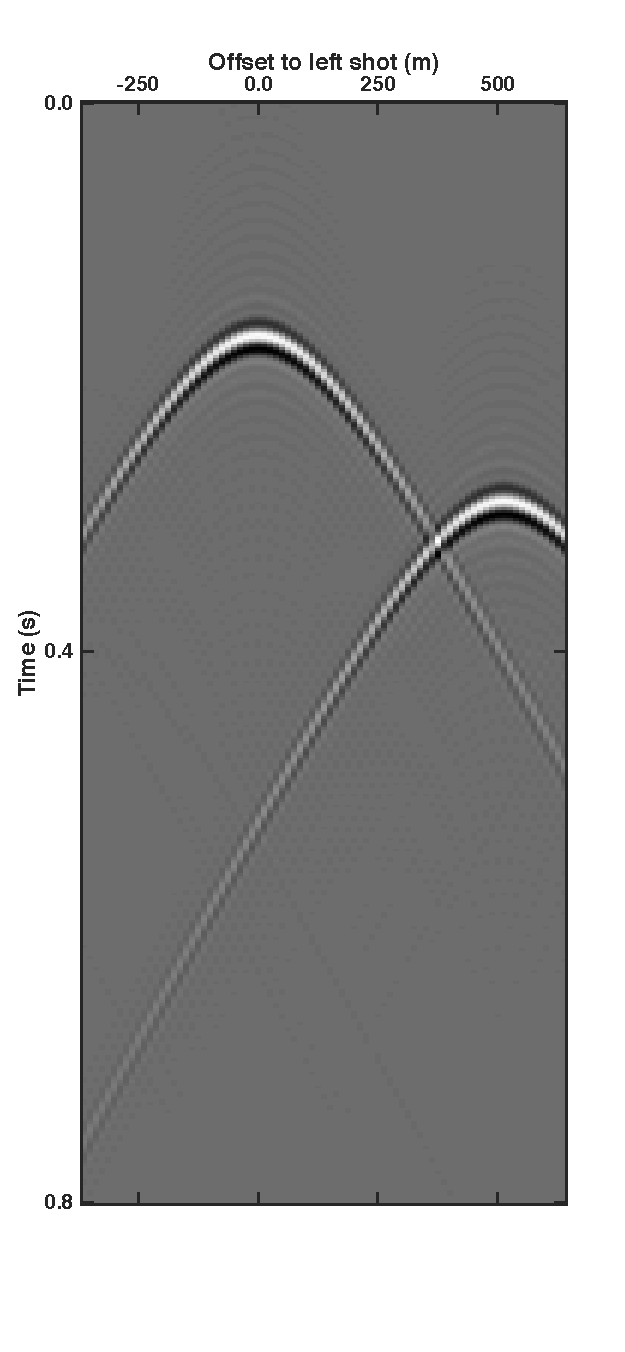
\includegraphics[width=0.25\textwidth]{Plots/Mahdad/30iter/BlendedCSG_sh1-edit_copy}
	\caption{Common shot gather of two blended shots. The shot on the right is fired \SI{120}{\milli\second} after the left shot.}
	\label{fig:Ch-Theory-BlendedData}
\end{figure}

Blending can be captured in the forward model by introducing a blending matrix, $\mathbf{\Gamma}$, which transforms the source matrix, $\mathbf{S}$, into a blended source matrix, $\mathbf{S}_{bl}$,

\begin{equation}
	\mathbf{S}_{bl} = \mathbf{S \, \Gamma}.
	\label{eq:Ch-Theory-BlendedSource}
\end{equation}

 Each row of $\mathbf{\Gamma}$ represents one source, and each column of $\mathbf{\Gamma}$ represents one experiment (see Figure \ref{fig:Ch-Theory-BlendedSource}). 
 
 The blending matrix captures the physics of a blended acquisition as follows: An element $\gamma_{ij}$ of the blending matrix includes a source $i$ and an experiment $j$. If the source $i$ is not fired in the $j^{th}$ experiment the amplitude $A_{ij}$ is zero. If it is fired, source $i$ has a relative amplitude $A_{ij}$ and a relative time delay $t_{ij}$ with respect to the first source fired in the $j^{th}$ experiment;

\begin{equation}
	\gamma_{ij} =  A_{ij} \mathrm{e}^{-j \omega \Delta t_{ij}}.
	\label{eq:Ch-Theory-BlendingElement}
\end{equation}  
 
Thus, the blending matrix selects specific sources from the source matrix and superimposes as visualized in Figure \ref{fig:Ch-Theory-BlendedSource}. From Figure \ref{fig:Ch-Theory-BlendedSource} it also becomes clear that both the blending matrix, $\mathbf{\Gamma}$, and the blended source matrix, $\mathbf{S}_{bl}$, have more rows than columns, i.e. there are more sources than experiments. Thus, the acquisition can be done in less time.

In the case of source blending the receiver matrix, $\mathbf{D}$, is not influenced by blending. And of course, the earth impulse response, $\mathbf{X}$, is independent of the acquisition design. Hence, the blended data can be written as;

\begin{equation}
	\mathbf{P}_{bl} = \mathbf{D} \, \mathbf{X} \, \mathbf{S}_{bl} = \mathbf{D} \, \mathbf{X} \, \mathbf{S} \, \mathbf{\Gamma} = \mathbf{P \, \Gamma}.
	\label{eq:Ch-Theory-BlendedData}
\end{equation}

Note that, the blended data matrix, $\mathbf{P}_{bl}$, also has less columns, i.e. less experiments, than the unblended data matrix, $\mathbf{P}$.



\section{Deblending} \label{sec:MahdadMethod}

Before removing the receiver matrix, $\mathbf{D}$, and the source matrix, $\mathbf{S}$, one must remove  the blending matrix, $\mathbf{\Gamma}$, from the blended data, $\mathbf{P}_{bl}$. This process is called deblending.

The deblending method presented in this thesis builds on the method of \citet{Mahdad-Deblending-Method}. Therefore, the method of \citet{Mahdad-Deblending-Method} is described in great detail.

The basic workflow of the method of \citet{Mahdad-Deblending-Method} is summarized in Figure \ref{fig:Ch-Theory-FlowChart} and will be explained step by step in the following subsections. 

\begin{figure}
	\centering
	\includegraphics[width=0.8\textwidth]{Plots/Mahdad-FlowChart-v5}
	\caption{Flowchart belonging to the deblending method of \citet{Mahdad-Deblending-Method}.}
	\label{fig:Ch-Theory-FlowChart}
\end{figure}

\subsection{Pseudo-Deblending}

Unfortunately, the inverse problem of equation \ref{eq:Ch-Theory-BlendedData} is underdetermined, which means that there is not a unique solution for the unblended data, $\mathbf{P}$. Thus, additional constraints are required to deblend the data, which are (1) sparsity of the signal in the $x$-$t$-domain and (2) coherency of the signal in the $f$-$k$-domain. 

The first estimate of the unblended data matrix, $\mathbf{P}$, is obtained by pseudo-deblending;

\begin{equation}
	\mathbf{P}_{ps} = \mathbf{P}_{bl} \, \mathbf{\Gamma}^H.
	\label{eq:Ch-Theory-PseudoDeblended}
\end{equation}

Pseudo-deblending copies the blended data to the locations of all shots present in the blended shot and shifts them  upward in time to compensate for the time delay. For example, Figure \ref{fig:Ch-Theory-PseudoDeblendedCSG2} and \ref{fig:Ch-Theory-PseudoDeblendedCSG} shows the two pseudo-deblended shot gathers of the blended data in Figure \ref{fig:Ch-Theory-BlendedData}. Note that the pseudo-deblended data have the same size as $\mathbf{P}$.


\subsection{Common Receiver Gather}
By transforming the data to another domain, e.g. to the common receiver domain, the interfering sources become incoherent and are visible as spiky noise (see Figure \ref{fig:Ch-Theory-PseudoDeblendedCRG}). Therefore, the interfering sources can be attenuated with a noise filter. 

%\todo[inline]{MOVE TO EXTENSION PART: Considering the 1/b factor, the interfering source creates blending noise and scales the amplitude of the shot of interest. So, is it correct to set blending noise and interfering source equal?}

\begin{figure}
	\centering
	\begin{subfigure}[t]{0.25\textwidth}
		\centering
		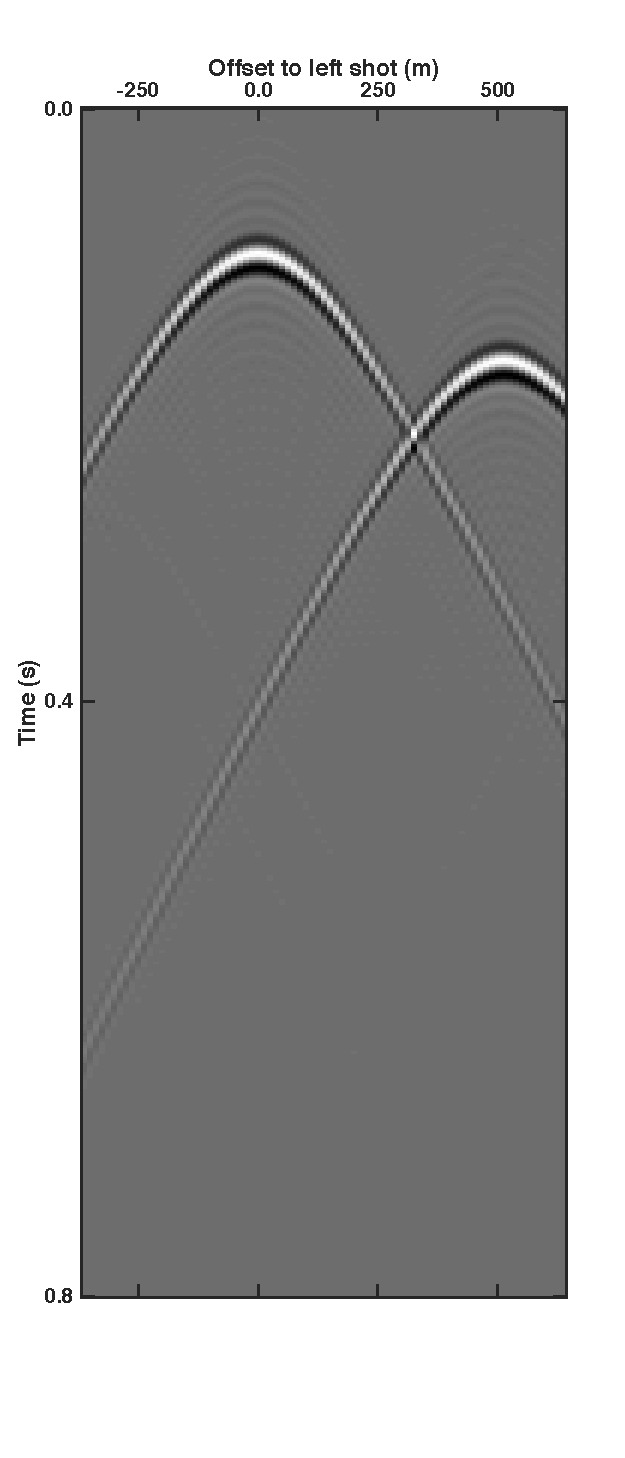
\includegraphics[width=0.925\textwidth]{Plots/Mahdad/30iter/Pseudo-DeblendedCSG_sh2}	
		\caption{Common-shot-gather}
		\label{fig:Ch-Theory-PseudoDeblendedCSG2}
	\end{subfigure}
	%
	\centering
	\begin{subfigure}[t]{0.25\textwidth}
		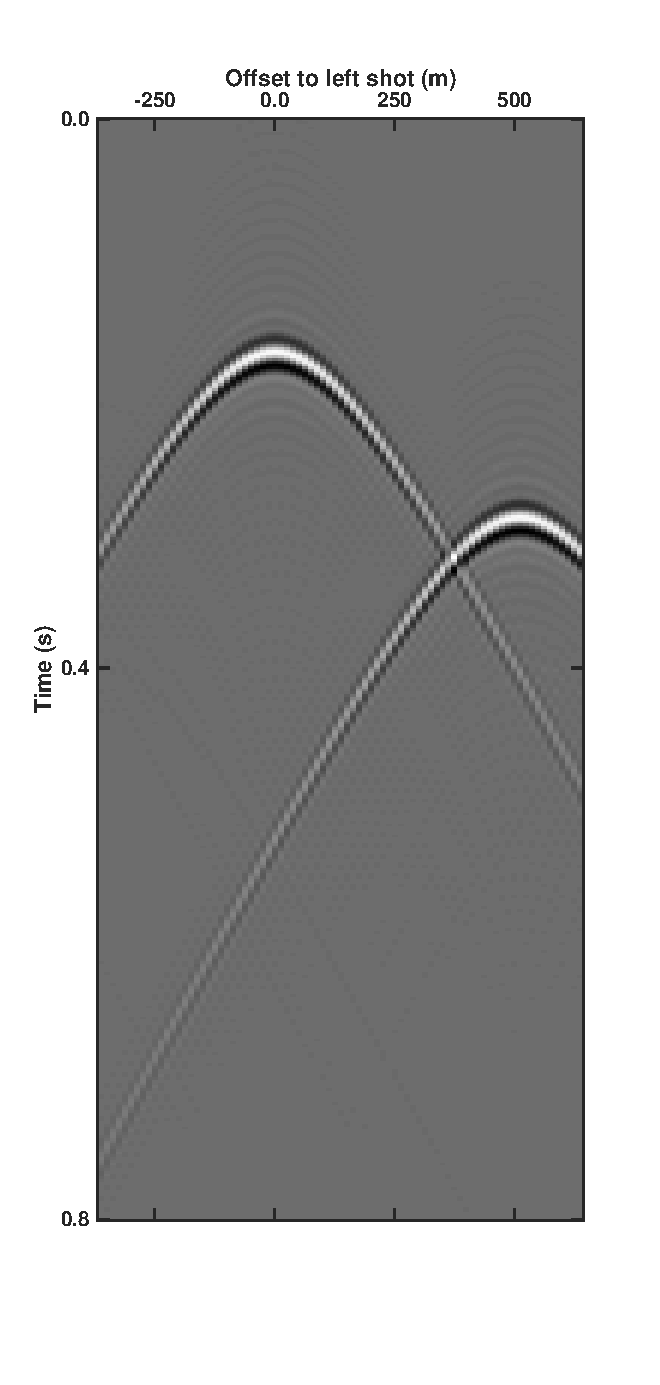
\includegraphics[width=\textwidth]{Plots/Mahdad/30iter/Pseudo-DeblendedCSG_sh1}	
		\caption{Common-shot-gather}
		\label{fig:Ch-Theory-PseudoDeblendedCSG}
	\end{subfigure}
	%
	\centering
	\begin{subfigure}[t]{0.25\textwidth}
		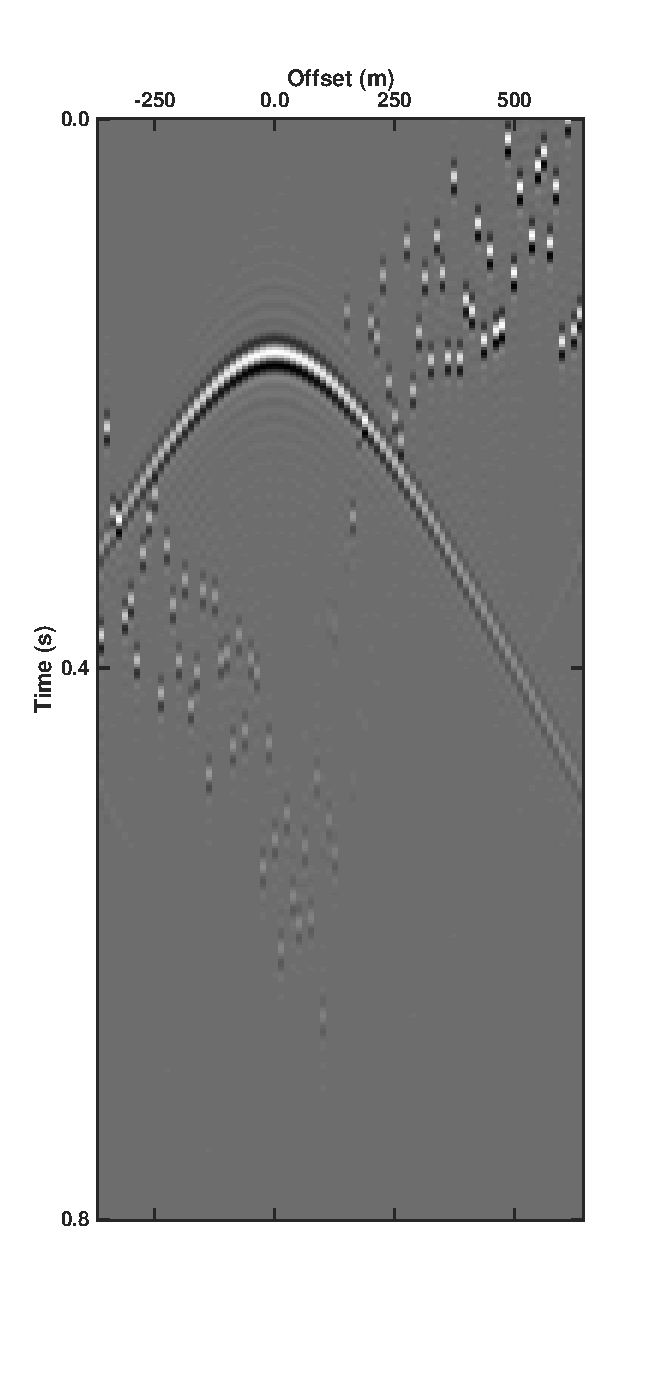
\includegraphics[width=\textwidth]{Plots/Mahdad/30iter/Pseudo-DeblendedCRG_rec30}	
		\caption{Common-receiver-gather}
		\label{fig:Ch-Theory-PseudoDeblendedCRG}
	\end{subfigure}
	\caption{Pseudo-deblended data, $\mathbf{P}_{ps}$, sorted in common shot gathers (a,b) and in a common receiver gather (c). The pseudo-deblended data of the right shot (a) and the left shot (b,c) were shifted by different time delays. The overlapping sources map in the pseudo-deblended shot gathers as coherent events, while they map as incoherent spikes in the pseudo-deblended receiver gather.}
	\label{fig:Ch-Theory-PseudoDeblended}

\end{figure}


\subsection{Iterative Blending Noise Estimation} \label{sec:IterBlenNoiseEst}

In an ideal case the noise generated by the interfering sources, the so called blending noise, is calculated with the unblended data,

\begin{equation}
	\mathbf{N} = \mathbf{P}_{bl} \, \mathbf{\Gamma}^H - \mathbf{P} = \mathbf{P}_{ps} - \mathbf{P}.
	\label{eq:Ch-Theory-Noise}
\end{equation}

Obviously, in practice the unblended data is unknown and must be estimated by adding extra constraints. The loop shown in Figure \ref{fig:Ch-Theory-FlowChart} applies the constraints to reduce the blending noise iteratively until the solution is obtained. 

In the following all the quantities which are estimated are indicated with a hat. The steps of the iterative blending noise estimation are demonstrated in Figure \ref{fig:Ch-Theory-IterativeDeblending}.

\begin{figure}
	\centering
	\begin{subfigure}[t]{0.25\textwidth}
		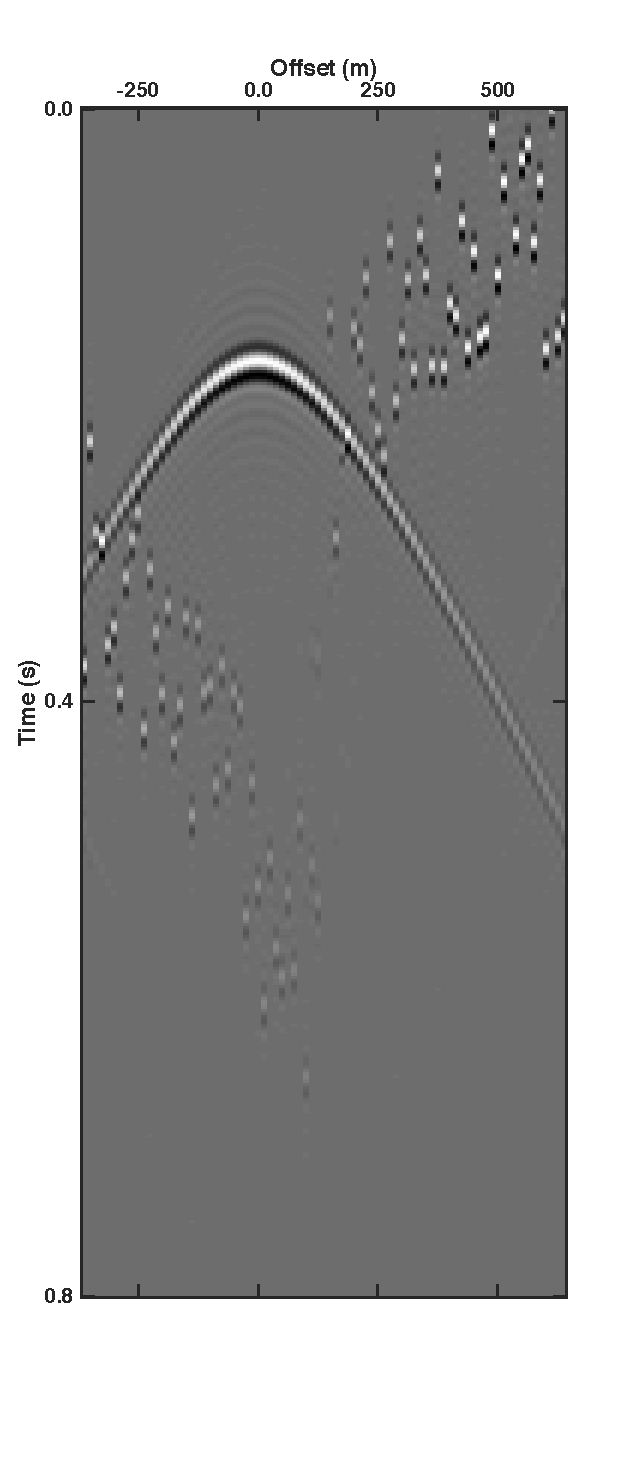
\includegraphics[width=\textwidth]{Plots/Mahdad/5iter/Pseudo-DeblendedCRG_rec30}	
		\caption{}
		\label{fig:Ch-Theory-PseudoDeblendedCRG5}
	\end{subfigure}
	%
	\centering
	\begin{subfigure}[t]{0.25\textwidth}
		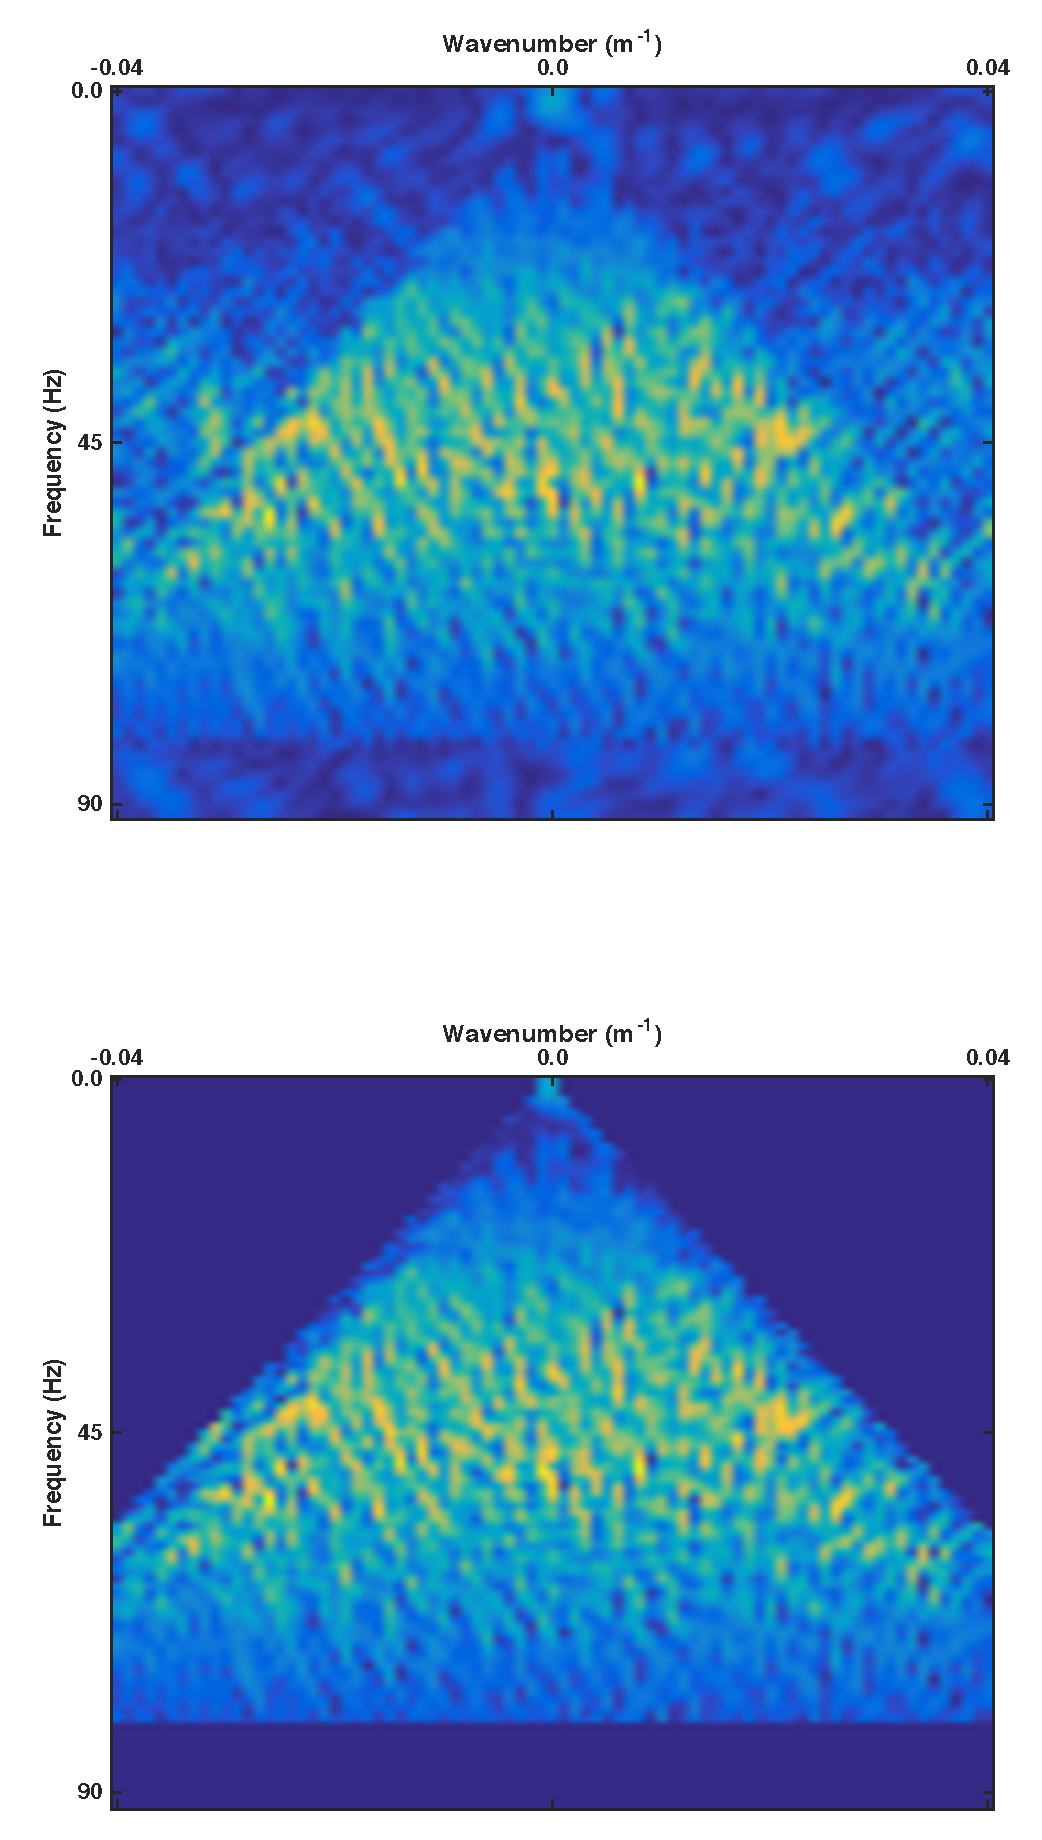
\includegraphics[width=\textwidth]{Plots/Mahdad/5iter/FK-Spectra}	
		\caption{}
		\label{fig:Ch-Theory-FKDeblended-NoFilter}
	\end{subfigure}
	%
	\begin{subfigure}[t]{0.25\textwidth}
		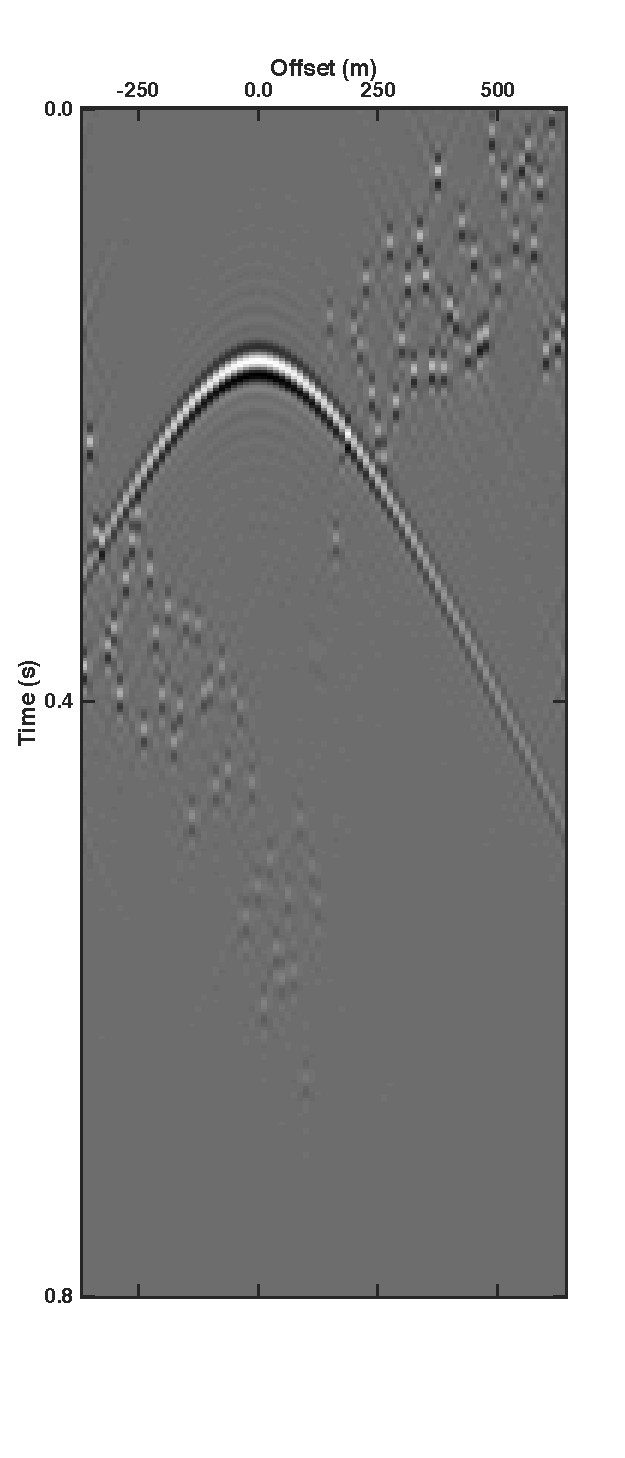
\includegraphics[width=\textwidth]{Plots/Mahdad/5iter/FkFilteredCRG_rec30}	
		\caption{}
		\label{fig:Ch-Theory-FKFiltered}
	\end{subfigure}
	%
	\begin{subfigure}[t]{0.25\textwidth}
		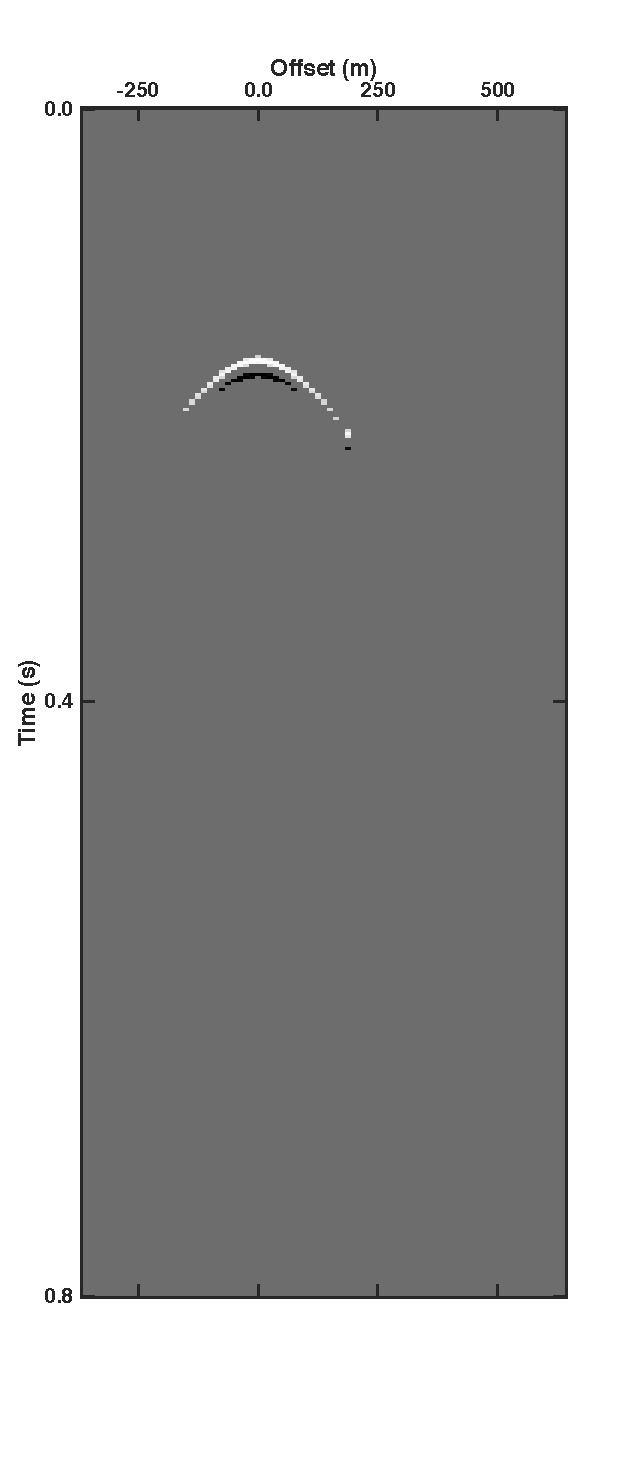
\includegraphics[width=\textwidth]{Plots/Mahdad/5iter/ThresholdCRG_rec30}	
		\caption{}
		\label{fig:Ch-Theory-Threshold}
	\end{subfigure}
	%
	\begin{subfigure}[t]{0.25\textwidth}
		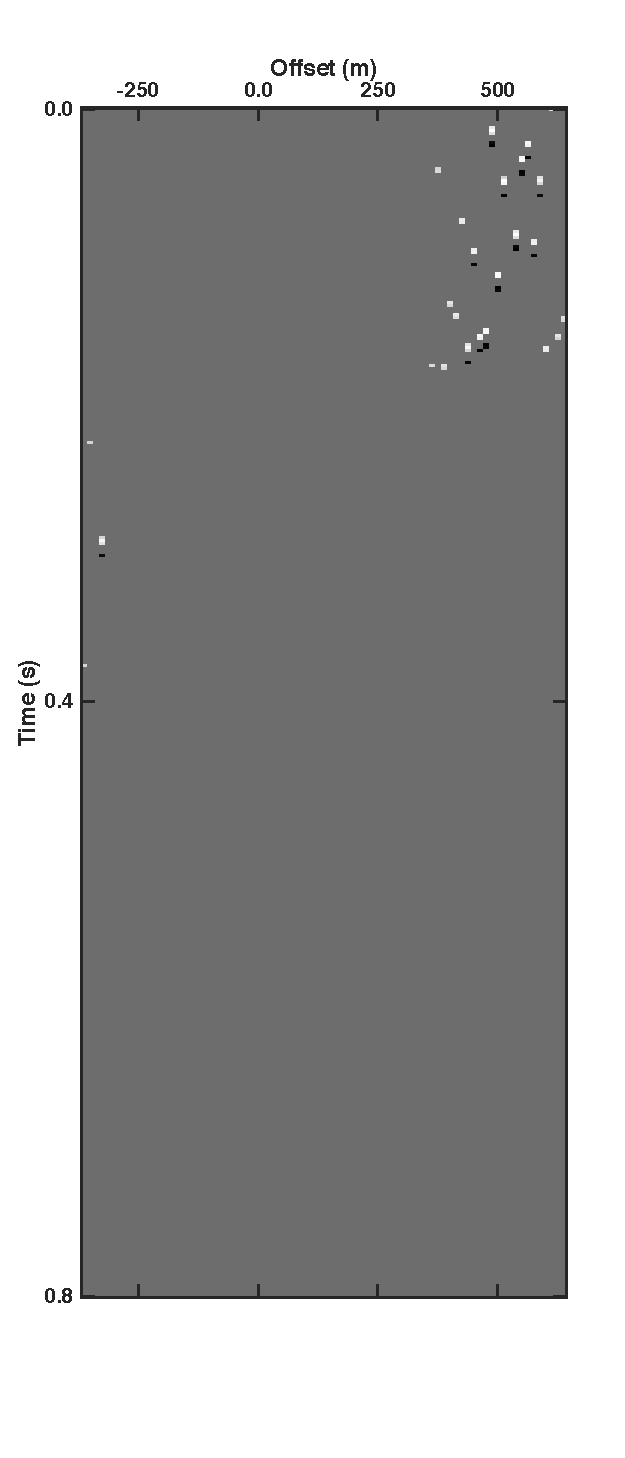
\includegraphics[width=\textwidth]{Plots/Mahdad/5iter/NoiseCRG_rec30}	
		\caption{}
		\label{fig:Ch-Theory-Noise}
	\end{subfigure}
	%
	\begin{subfigure}[t]{0.25\textwidth}
		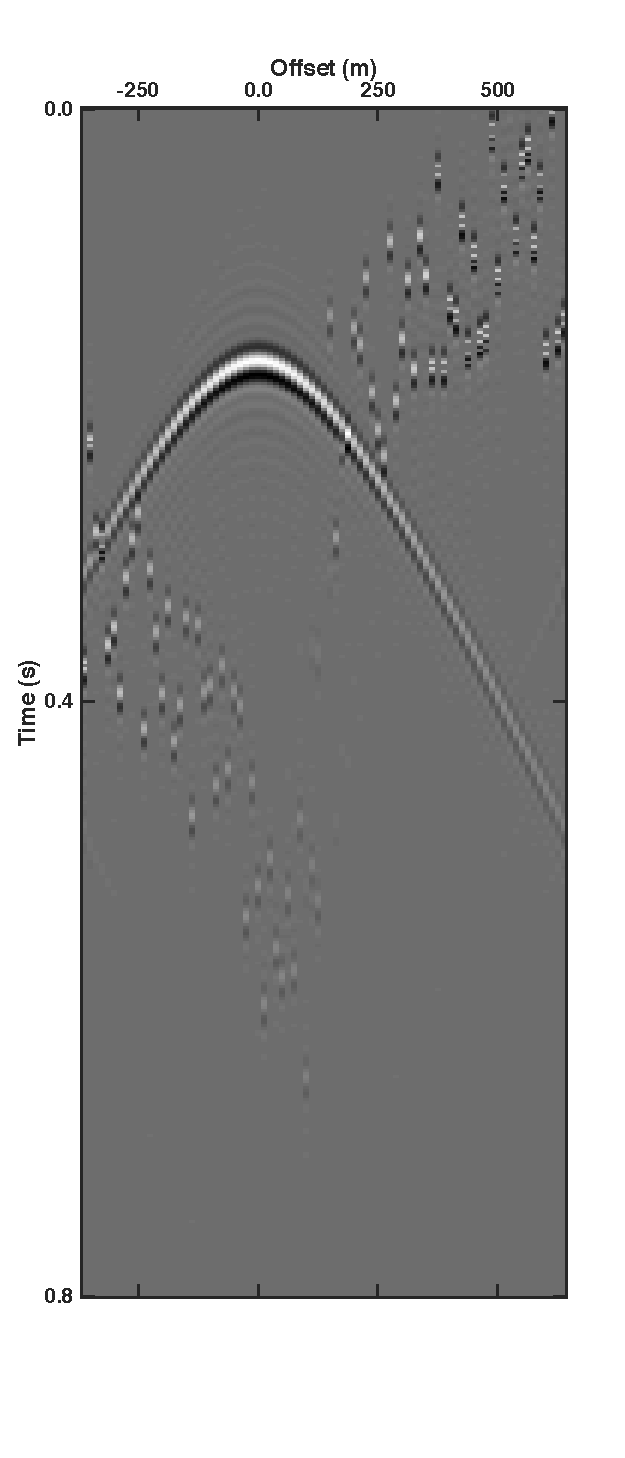
\includegraphics[width=\textwidth]{Plots/Mahdad/5iter/DeblendedCRG_rec30}	
		\caption{}
		\label{fig:Ch-Theory-Deblended}
	\end{subfigure}
	\caption{(a) Pseudo-deblended receiver gather. The subfigures (b)-(f) illustrate each step of the deblending algorithm. For better visibility examples from the $5^{th}$ iteration are chosen. (b) $f$-$k$-spectrum before (top) and after (bottom) $f$-$k$-filtering, (c) $f$-$k$-filtered common receiver gather, (d) after thresholding, (e) estimated source interference (f) estimated data.}
	\label{fig:Ch-Theory-IterativeDeblending}
\end{figure}


\subsubsection*{F-K-Filtering}

One of the constraints is coherency, i.e. by assuming the blending noise in Figure \ref{fig:Ch-Theory-PseudoDeblendedCRG} is incoherent it can be removed. For this purpose the data is transformed from the space time to the wavenumber frequency domain where the spiky noise spreads over all wavenumber and frequency components (see Figure \ref{fig:Ch-Theory-FKDeblended-NoFilter}, top). 

%For a 2D $f$-$k$-spectrum the minimum (physical) velocity of the subsurface, $v_{min}$, determines the maximum wavenumber, $k_{max}$,  for a given frequency, $f$;

The unblended data maps in the $f$-$k$-domain as a cone (see Figure \ref{fig:Ch-Theory-fk-Unblended-data}). The minimum (physical) velocity, $v_{min}$, of the subsurface determines the slope of the cone. This means that for a given frequency, $f$, the maximum wavenumber, $k_{max}$, is defined as; 

\begin{equation}
	k_{max} = \frac{f}{v_{min}}.
	\label{eq_Ch-Theory-MaxWavenmber}
\end{equation} 

In the marine case the minimum velocity is usually the water velocity, $v_{w} = \SI{1500}{\metre\per\second}$.

\begin{figure}
	\centering
	\begin{subfigure}[t]{0.45\textwidth}
		\centering
		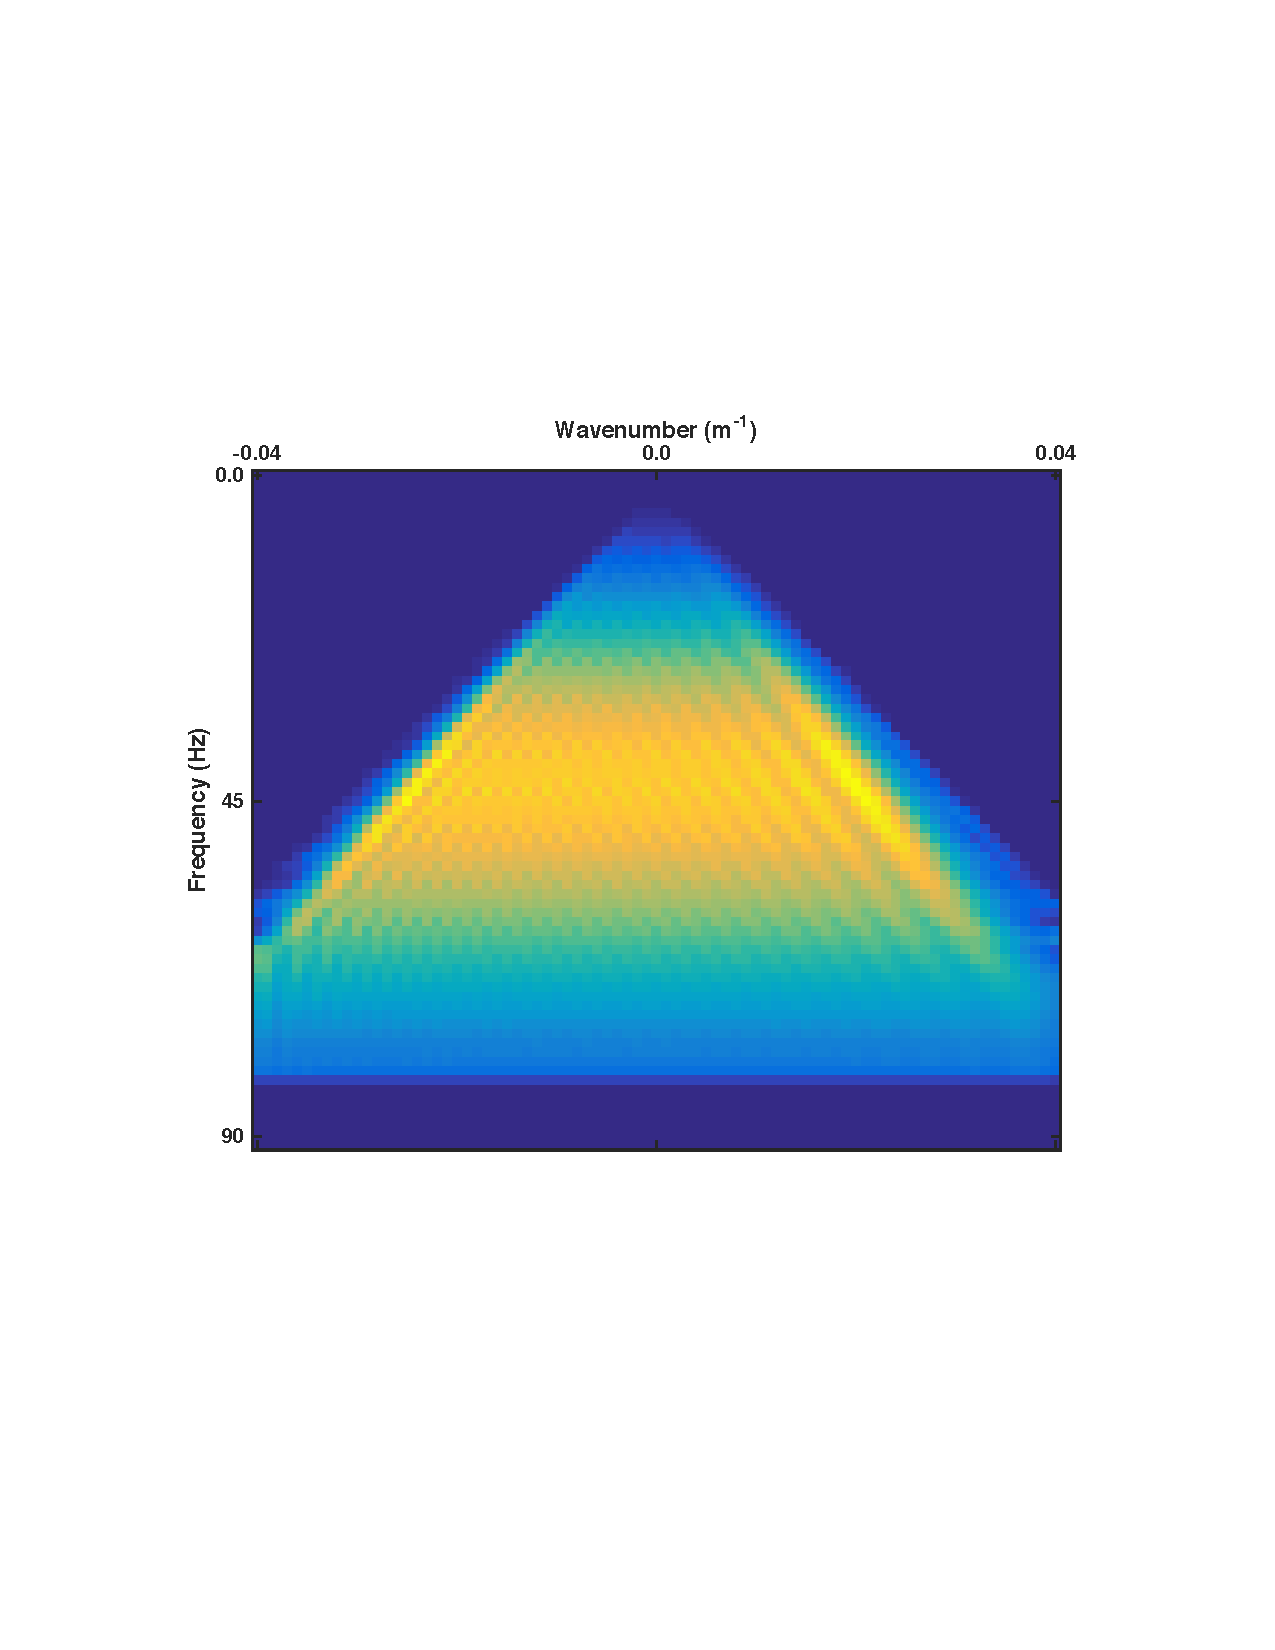
\includegraphics[width = \textwidth]{Plots/Mahdad/30iter/FK-UnblendedCRG_r1}
		\caption{$f$-$k$-spectrum of an unblended common shot gather.}
		\label{fig:Ch-Theory-fk-Unblended-data}
	\end{subfigure}
	%
	\centering
	\begin{subfigure}[t]{0.45\textwidth}
		\centering
		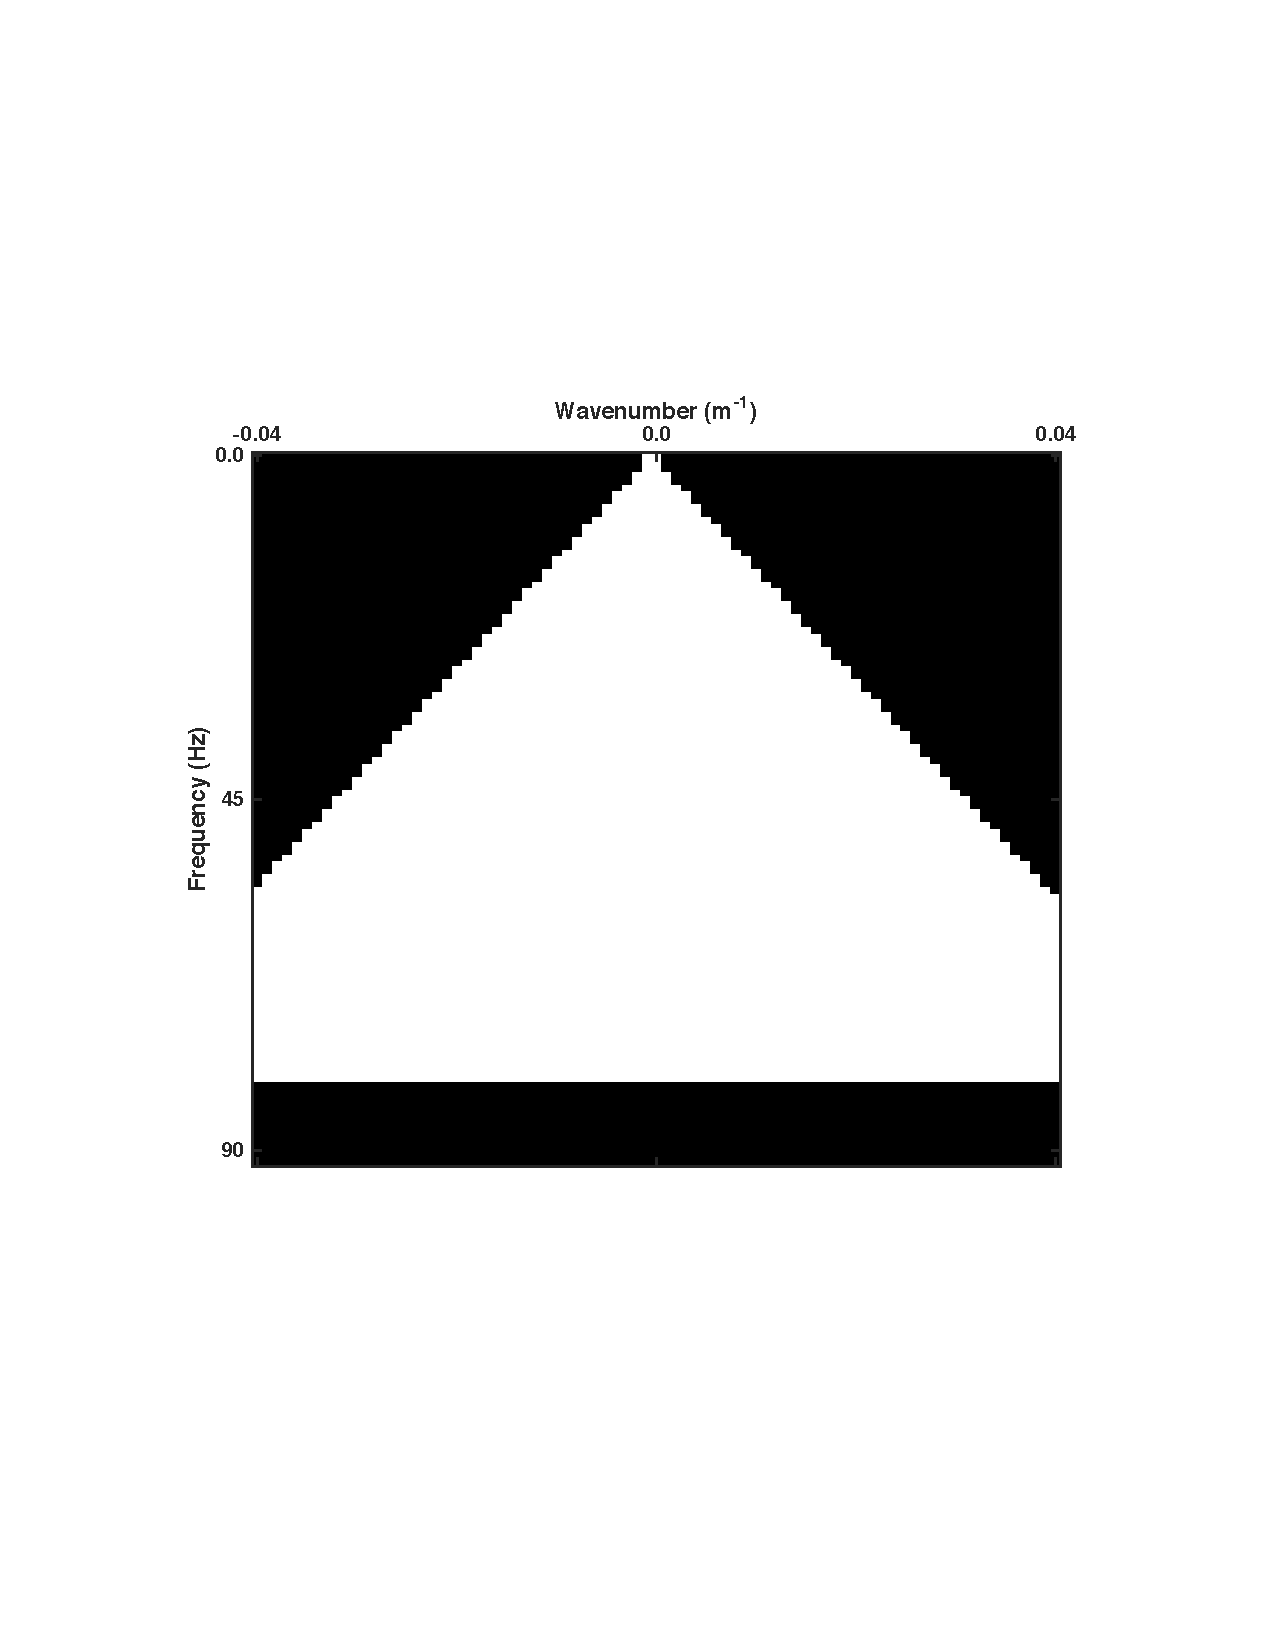
\includegraphics[width = 0.957\textwidth]{Plots/Mahdad/5iter/FK-MaskCRG_rec30}
		\caption{The $f$-$k$-mask is determined by the minimum signal velocity in the subsurface. The white area of the filter equals one, the black area equals zero. Thus, the filter removes data which is mapped outside of the white signal cone.}
		\label{fig:Ch-Theory-FK-Mask}
	\end{subfigure}
	
	\caption{}
	\label{fig:Ch-Theory-fk-unblended-data-mask}
\end{figure}

For each frequency, $f$, wavenumbers above $k_{max}$ are removed which results in a 2D $f$-$k$-filter as depicted in Figure \ref{fig:Ch-Theory-FK-Mask}.

The $f$-$k$-filter removes the part of the blending noise, which maps outside of the signal cone. Thus, after transforming the data back to the space time domain the amplitudes of the spiky noise are attenuated (see Figure \ref{fig:Ch-Theory-FKFiltered}). 

Note that $f$-$k$-filtering can only reduce unaliased frequency components of the blending noise. In Figure \ref{fig:Ch-Theory-FK-Mask} the highest unaliased frequency is defined by the point where the white cone intersects with the frequency axis, i.e. at \SI{60}{\hertz}. 

The high cut frequency of the $f$-$k$-mask is set according to the highest frequency components in the data. The aliased blending noise will pass the $f$-$k$-filter and will be reduced afterwards by thresholding. 


\subsubsection*{Thresholding}

The second constraint for the estimation of the unblended data is sparsity of the signal in the space time domain.

After $f$-$k$-filtering the spiky noise is attenuated (see Figure \ref{fig:Ch-Theory-FKFiltered}). Consequently, the signal amplitudes are now stronger than the noise amplitudes. This allows to define a threshold in the $x$-$t$ domain, which is larger than the noise amplitudes and smaller than the highest signal amplitudes. Only amplitudes above the threshold are picked, i.e. only signal with strong amplitudes is selected (see Figure \ref{fig:Ch-Theory-Threshold}). 

\subsubsection*{Interference Estimation}

The resulting thresholded data, \textbf{\={P}}, is used to predict the source interference;

\begin{equation}
	\textbf{\^{N}}_\textbf{i} = \textbf{\={P}} \, (\mathbf{\Gamma \, \Gamma^H} - \textbf{I}),
	\label{eq:Ch-Theory-NoiseEstimation}
\end{equation}

which is illustrated in Figure \ref{fig:Ch-Theory-Noise}.

At each iteration the blending noise is attenuated further, such that the threshold can be lowered. Hence, the predicted source interference increases and approaches the true source interference. 


\subsubsection*{Blending Noise Subtraction} 

The estimate of the unblended data matrix \textbf{\^{P}}$_\textbf{i}$ is updated by subtracting the noise from the pseudo-deblended data,

\begin{equation}
	\textbf{\^P}_\textbf{i+1} = \textbf{P}_\textbf{bl} \, \mathbf{\Gamma}^H - \textbf{\^{N}}_\textbf{i}, 
	\label{eq:Ch-Theory-DataUpdate1}
\end{equation}

which is shown in Figure \ref{fig:Ch-Theory-Deblended}.

This process is repeated iteratively till convergence is reached. In this context convergence can be defined as the point where the difference $\mid \textbf{\^P}_\textbf{i+1} - \textbf{\^{P}}_\textbf{i} \mid$ drops below a predefined limit. Alternatively, one can set a maximum number of iterations. 

Figure \ref{fig:Ch-Theory-EstimatedData} shows the estimate of the unblended data for increasing iterations. One can observe that the blending noise is attenuated with every iteration, and the blended shot is successively  attenuated.

Note that $f$-$k$-filtering lowers the noise level by removing unaliased blending noise. Next, the lowered noise level enables thresholding to reduce aliased frequency components of the blending noise. Thus, the combination of $f$-$k$-filtering and thresholding is very powerful.


\begin{figure}
	\centering
	\begin{subfigure}[t]{0.25\textwidth}
		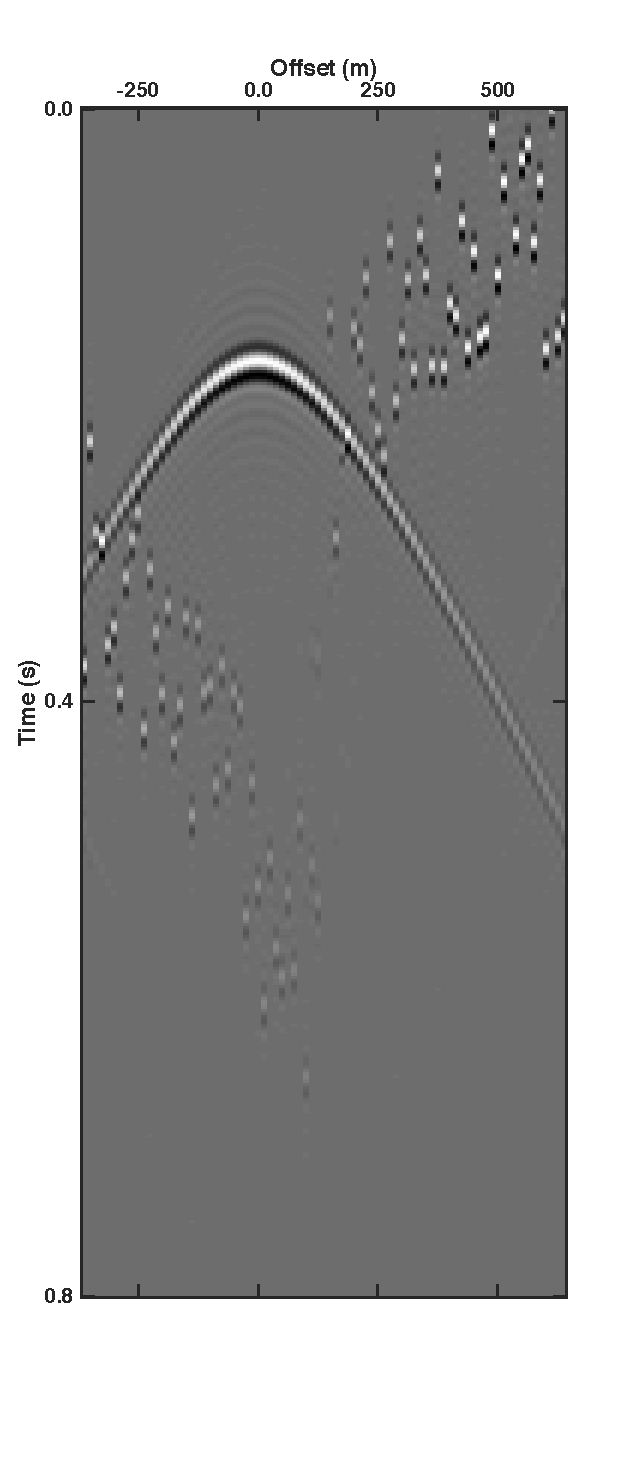
\includegraphics[width=\textwidth]{Plots/Mahdad/1iter/DeblendedCRG_rec30}	
		\caption{1 Iteration}
		\label{fig:Ch-Theory-DeblendedCRG1}
	\end{subfigure}
	%
	\centering
	\begin{subfigure}[t]{0.25\textwidth}
		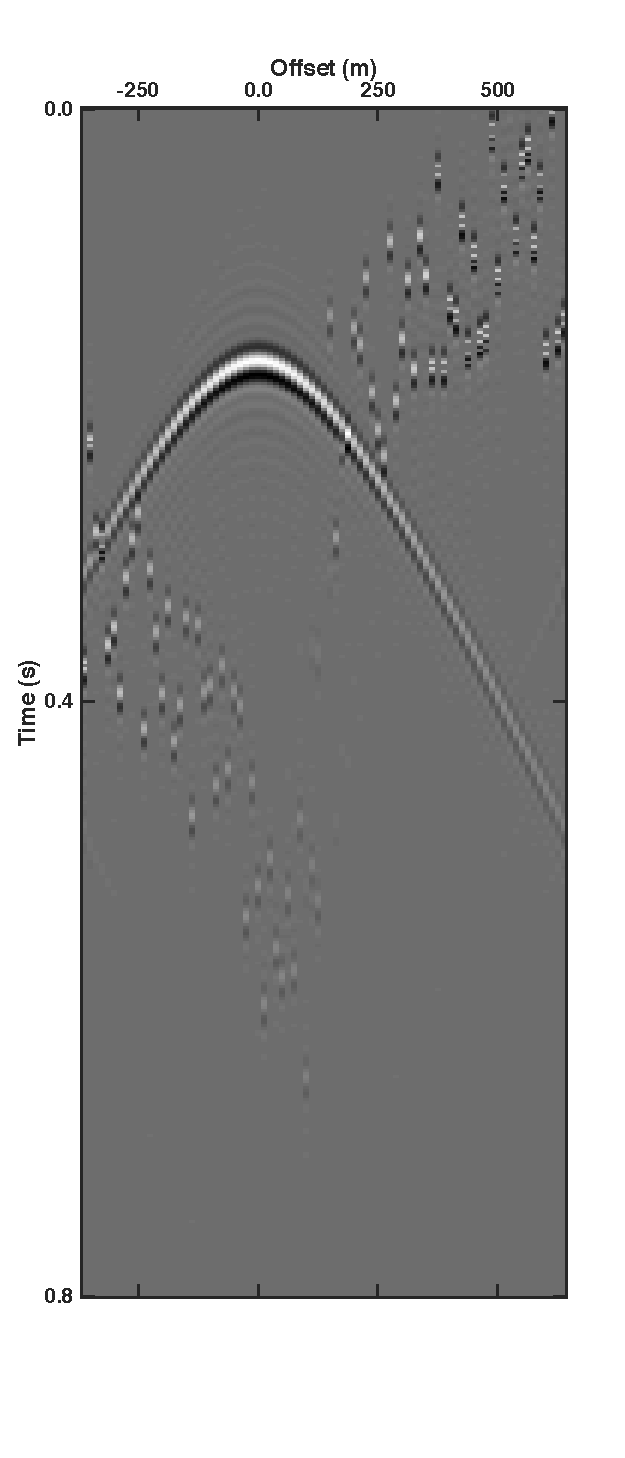
\includegraphics[width=\textwidth]{Plots/Mahdad/5iter/DeblendedCRG_rec30}	
		\caption{5 Iterations}
		\label{fig:Ch-Theory-DeblendedCRG5}
	\end{subfigure}
	%
	\begin{subfigure}[t]{0.25\textwidth}
		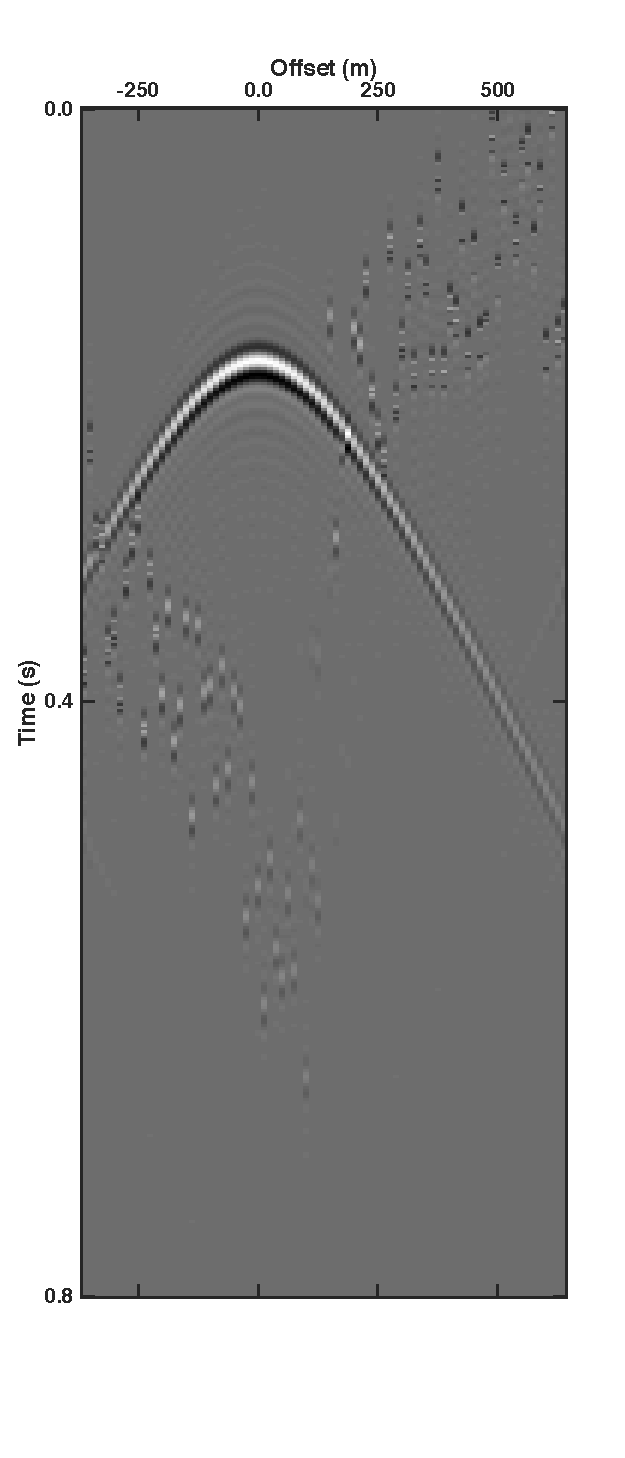
\includegraphics[width=\textwidth]{Plots/Mahdad/10iter/DeblendedCRG_rec30}	
		\caption{10 Iterations}
		\label{fig:Ch-Theory-DeblendedCRG10}
	\end{subfigure}
	%
	\begin{subfigure}[t]{0.25\textwidth}
		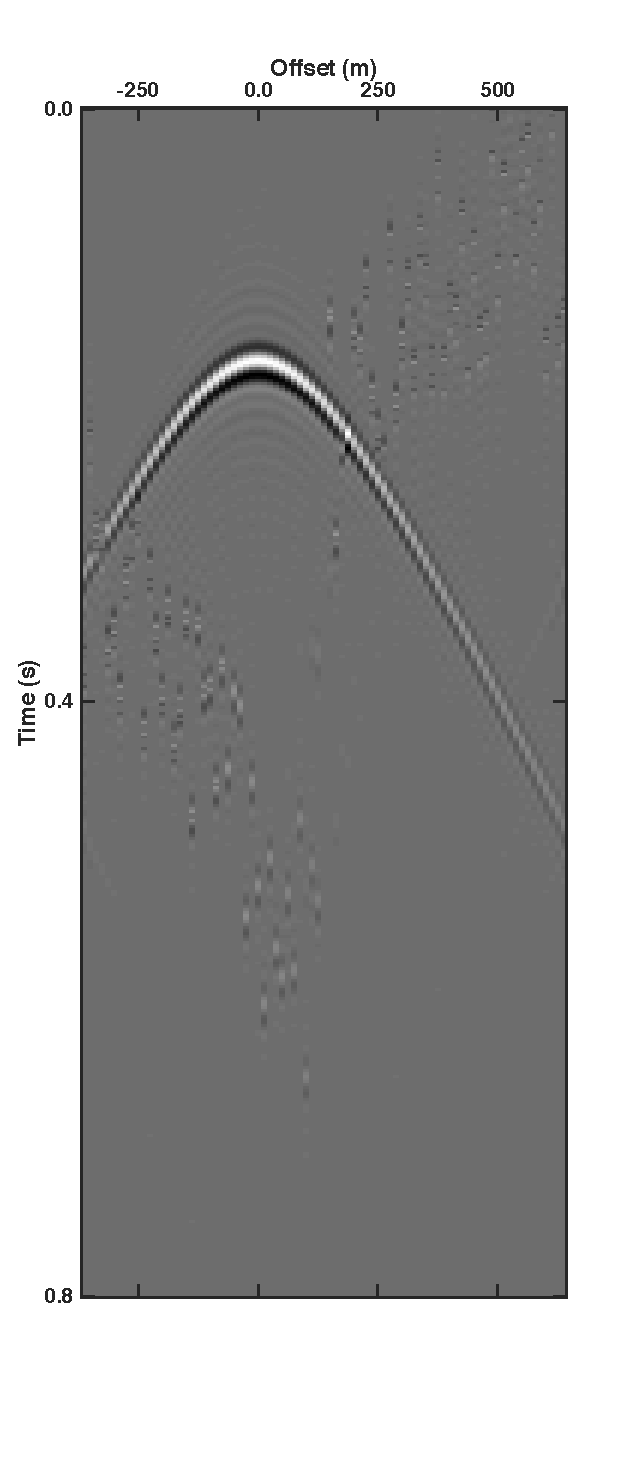
\includegraphics[width=\textwidth]{Plots/Mahdad/15iter/DeblendedCRG_rec30}	
		\caption{15 Iterations}
		\label{fig:Ch-Theory-DeblendedCRG15}
	\end{subfigure}
	%
	\begin{subfigure}[t]{0.25\textwidth}
		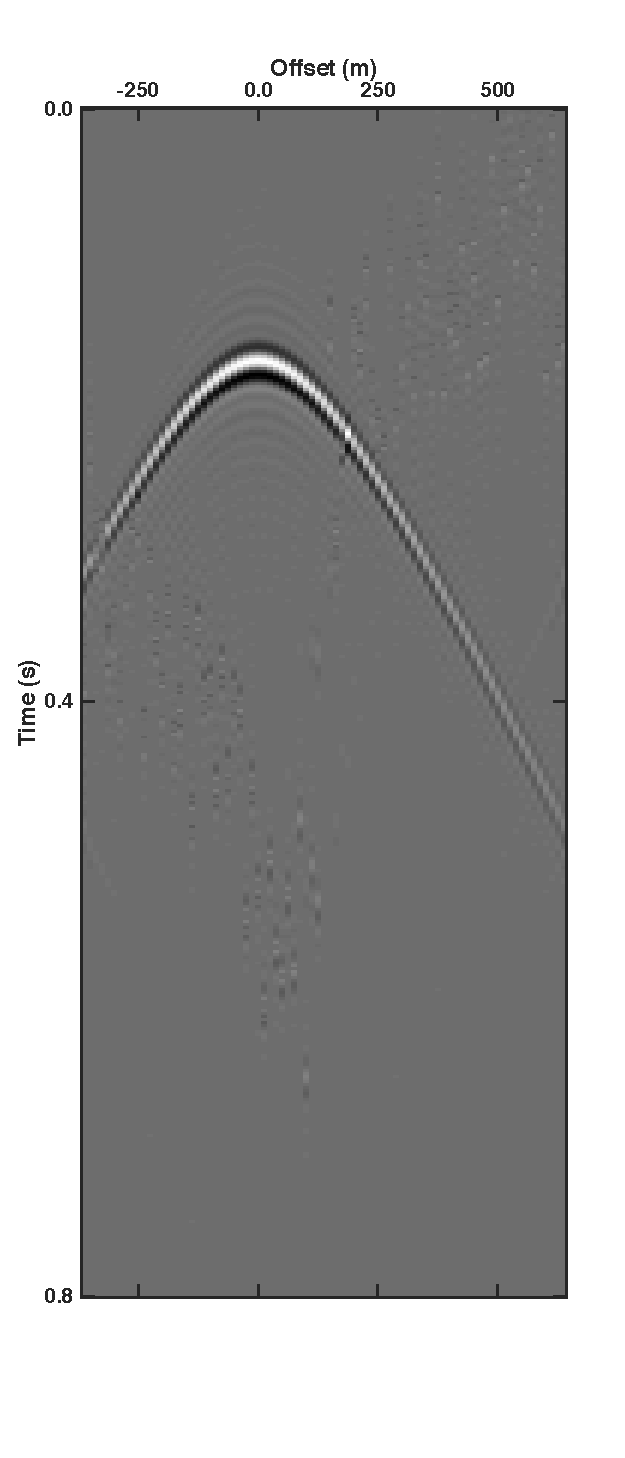
\includegraphics[width=\textwidth]{Plots/Mahdad/20iter/DeblendedCRG_rec30}	
		\caption{20 Iterations}
		\label{fig:Ch-Theory-DeblendedCRG20}
	\end{subfigure}
	%
	\begin{subfigure}[t]{0.25\textwidth}
		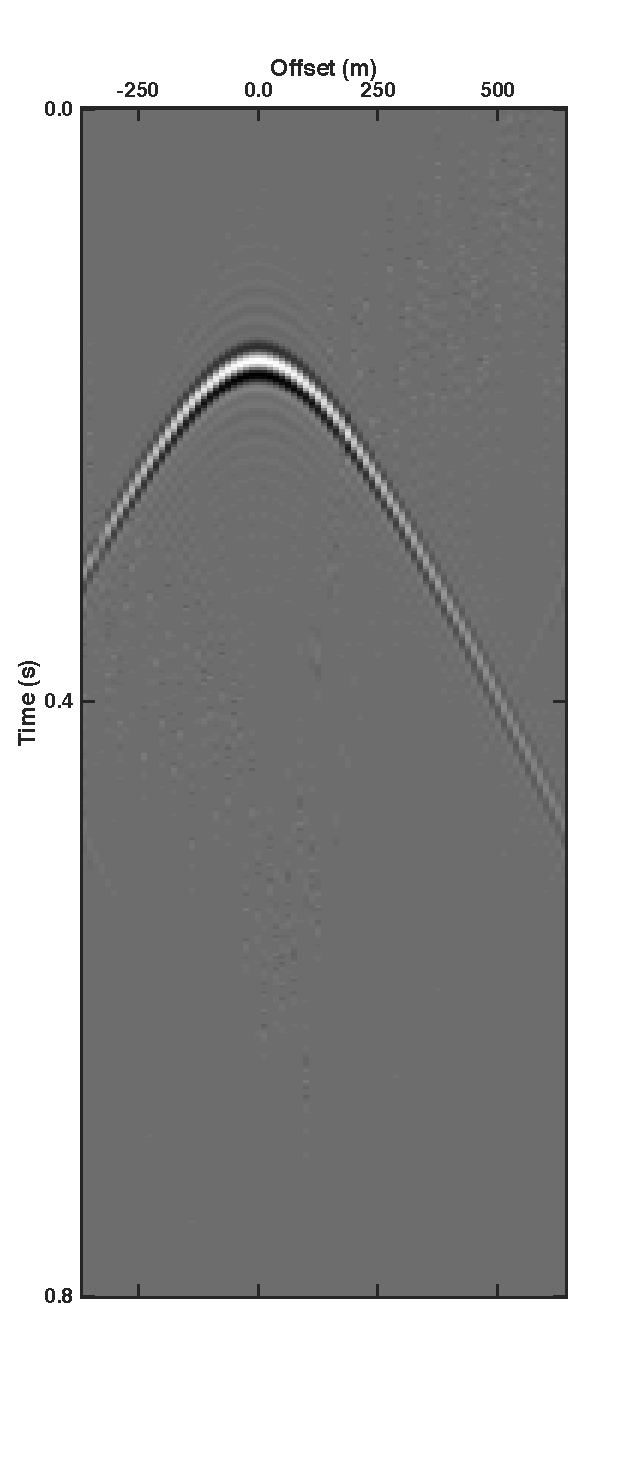
\includegraphics[width=\textwidth]{Plots/Mahdad/25iter/DeblendedCRG_rec30}	
		\caption{25 Iterations}
		\label{fig:Ch-Theory-DeblendedCRG25}
	\end{subfigure}
	\caption{Common receiver gather of the estimated data after 1, 5, 10, 15, 20 and 25 iterations.}
	\label{fig:Ch-Theory-EstimatedData}

\end{figure}

\FloatBarrier

\section{Analysis of the Blending Matrix} \label{sec:BlendingMatrix}

In order to optimize the blended acquisition design, one must understand the properties of the blending matrix $\mathbf{\Gamma}$ and its influence on the deblending performance.

The blending matrix $\mathbf{\Gamma}$ determines the pseudo-deblended data,

\begin{equation}
	\mathbf{ P_{ps} } = \mathbf{P \Gamma \Gamma ^H},
	\label{eq:Ch-Theory-Pseudo-Deblended-Data}
\end{equation}

which is a superposition of the unblended data, $\mathbf{P}$, and the source interference, $\mathbf{N}$,

\begin{equation}
	\mathbf{P}_{ps} = \mathbf{P} + \mathbf{N}.
	\label{eq:Ch-Theory-PseudoSuperposition}
\end{equation}

The more incoherent the source interference, $\mathbf{N}$, the better it can be removed by noise filters.

In the following the effect of the blending matrix, $\mathbf{\Gamma}$, on the product $\mathbf{\Gamma \Gamma}^H$ and on the pseudo-deblended data is analyzed. For simplicity, it is assumed that the blending matrix, $\mathbf{\Gamma}$, only contains phase shift terms, $\mathrm{e}^{-j \omega \Delta t}$, with an amplitude equal to 1 or 0. It is also assumed that each source is fired only once, unlike e.g. the shot repetition case \citep{Sixue}.

Each row of $\mathbf{\Gamma}$ represents a source $k$ and each column of $\mathbf{\Gamma ^H}$ represents a source $l$ with a complex conjugated phase term (see Figure \ref{fig:Ch-Theory-GGH}). Hence, each element $g_{kl}$ of the matrix $\mathbf{\Gamma \Gamma}^H$ is the dot product between the $k^{th}$ source and the complex conjugate of the $l^{th}$ source.

\begin{figure}
	\centering
	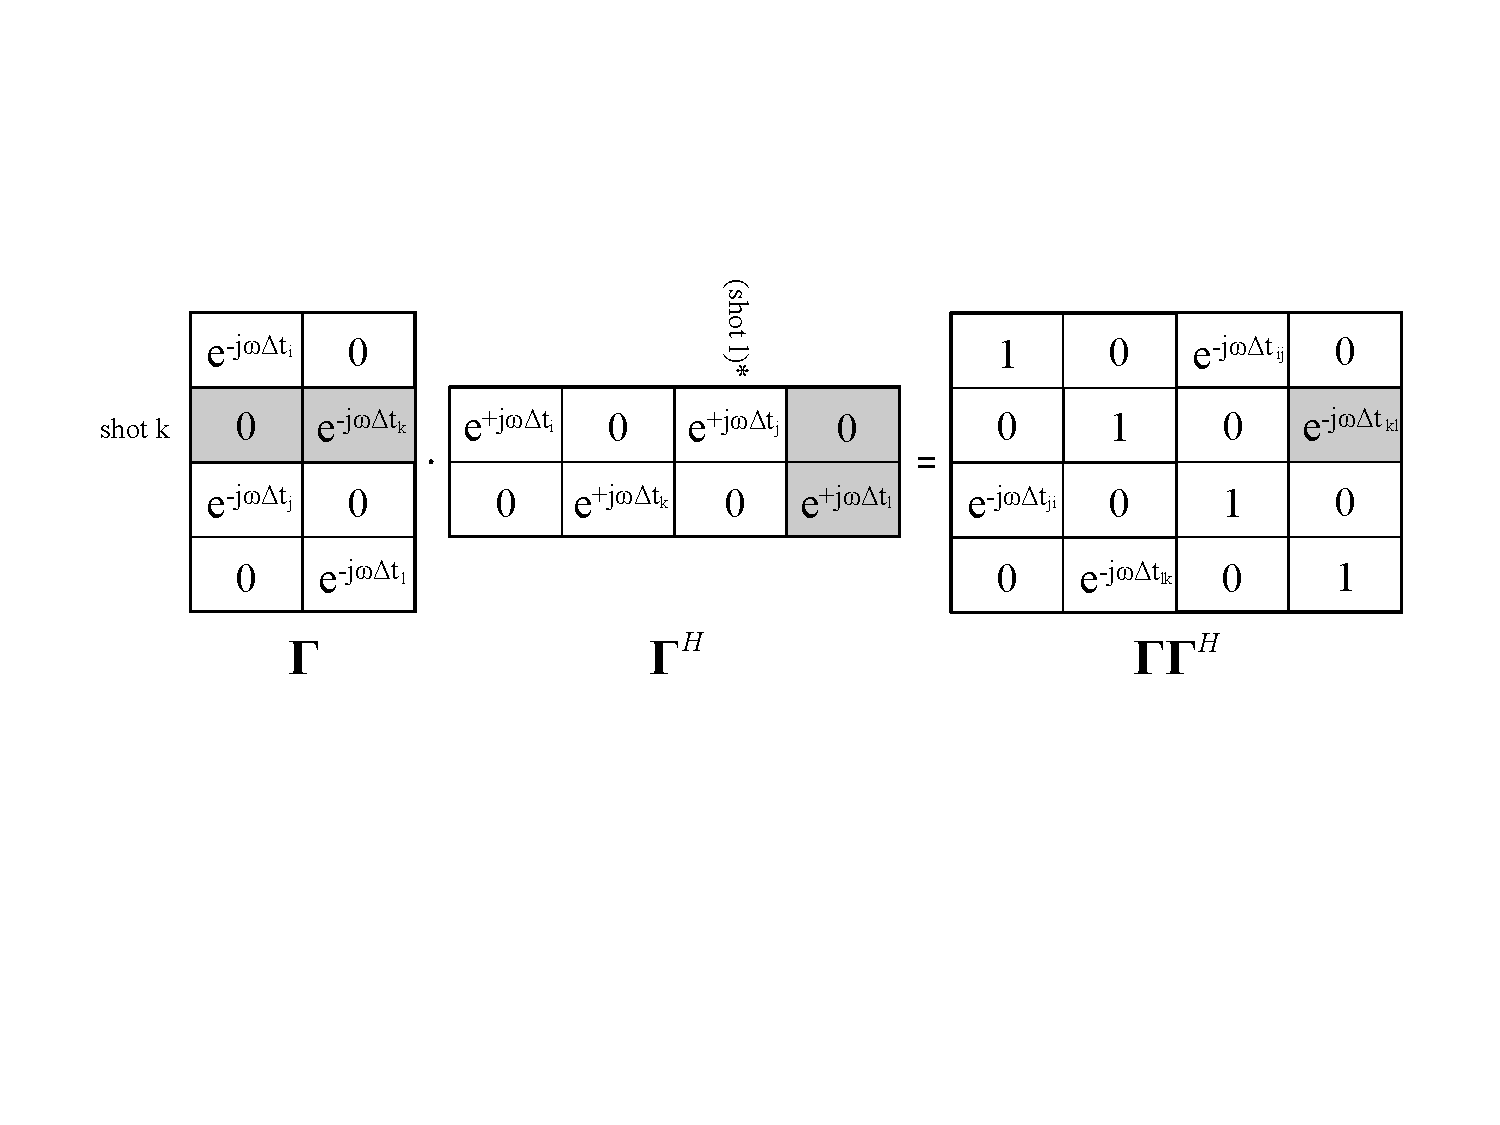
\includegraphics[width = \textwidth]{Plots/GGH}
	\caption{Illustration of the matrix product, $\mathbf{\Gamma \Gamma}^H$. In this notation $\Delta t_k$ refers to the phase shift of the source $k$, and $\Delta t_{kl}$ refers to the phase shift between the sources $k$ and $l$, $\Delta t_{kl} = \Delta t_k - \Delta t_l$.}
	\label{fig:Ch-Theory-GGH}
\end{figure}

Consequently, an element $g_{kl}$ of the product $\mathbf{\Gamma \Gamma}^H$ represents the overlap of the sources $k$ and $l$ for all experiments. The main diagonal of $\mathbf{\Gamma \Gamma}^H$ refers to the overlap of each source with itself, which of course is perfect and therefore equal to 1. The off diagonal elements of $\mathbf{\Gamma \Gamma}^H$ are either 0 if the associated sources do not overlap, or contain a phase shift, $\mathrm{e}^{\, -j \omega \Delta t_{kl}}$.

In equation \ref{eq:Ch-Theory-Pseudo-Deblended-Data} the main diagonal elements of $\mathbf{\Gamma \Gamma}^H$ copy the data matrix, $\mathbf{P}$, while the off-diagonal elements create the source interference, $\mathbf{N}$. If the elements $g_{ik}$ along a sub-diagonal are in phase, they will shift the columns of the data matrix and apply a coherent phase shift to each of them (see Figure \ref{fig:Ch-Theory-PseudoCRG-CoherentDelay}). Instead if the elements $g_{ik}$ along a sub-diagonal are out of phase, they will shift the columns of the data matrix and distort the phase of each column (see Figure \ref{fig:Ch-Theory-PseudoCRG-IncoherentDelay}). 

Figure \ref{fig:Ch-Theory-PseudoCRG-FK-CoherentDelay} and \ref{fig:Ch-Theory-PseudoCRG-FK-IncoherentDelay} display the $f$-$k$-spectra of the pseudo-blended data for constant and random firing time delays respectively. In the case of constant firing time delays almost all of the energy maps in the signal cone. In the case of random firing time delays a significant part of the energy maps outside of the signal cone. Therefore, the coherency constraint requires random firing delays.  

\begin{figure}
	\centering
	\begin{subfigure}[b]{0.3\textwidth}
		\centering
		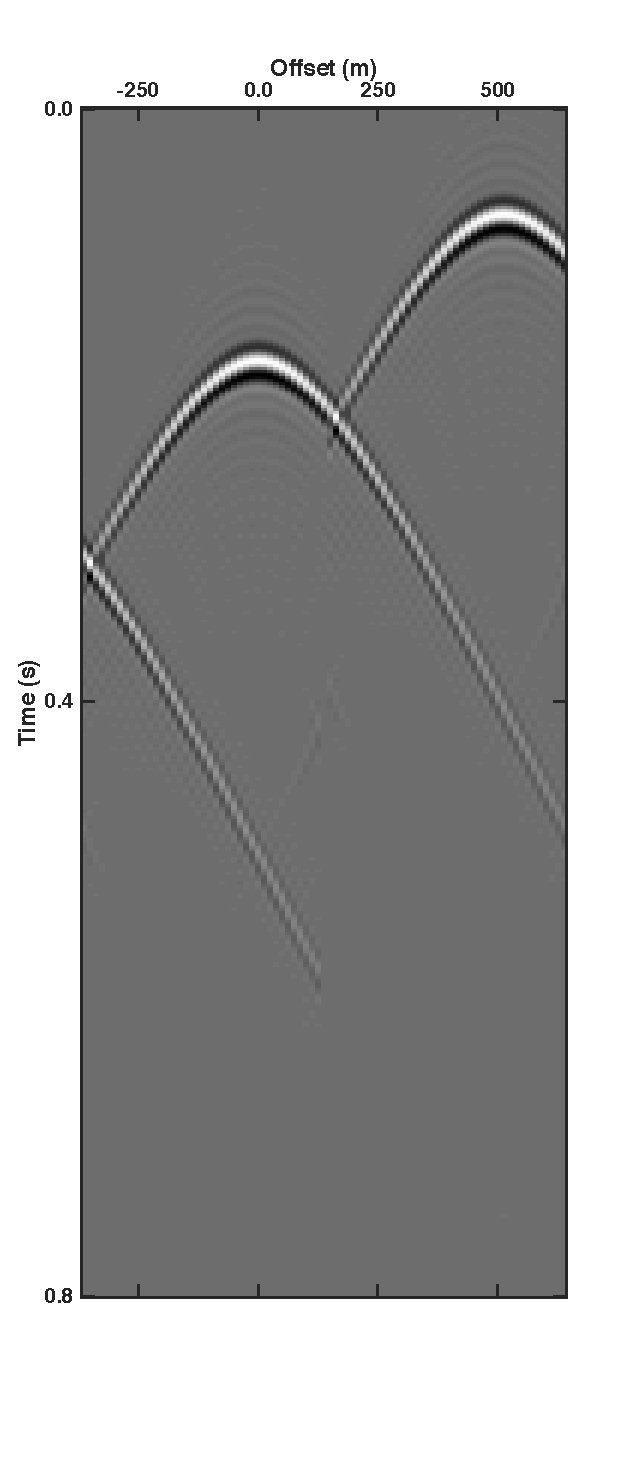
\includegraphics[width = \textwidth]{Plots/Mahdad/25iter/TimeDelay/Pseudo-DeblendedCRG_rec30_coh}
		\caption{}
		\label{fig:Ch-Theory-PseudoCRG-CoherentDelay}
	\end{subfigure}
	%
	\centering
	\begin{subfigure}[b]{0.3\textwidth}
		\centering
		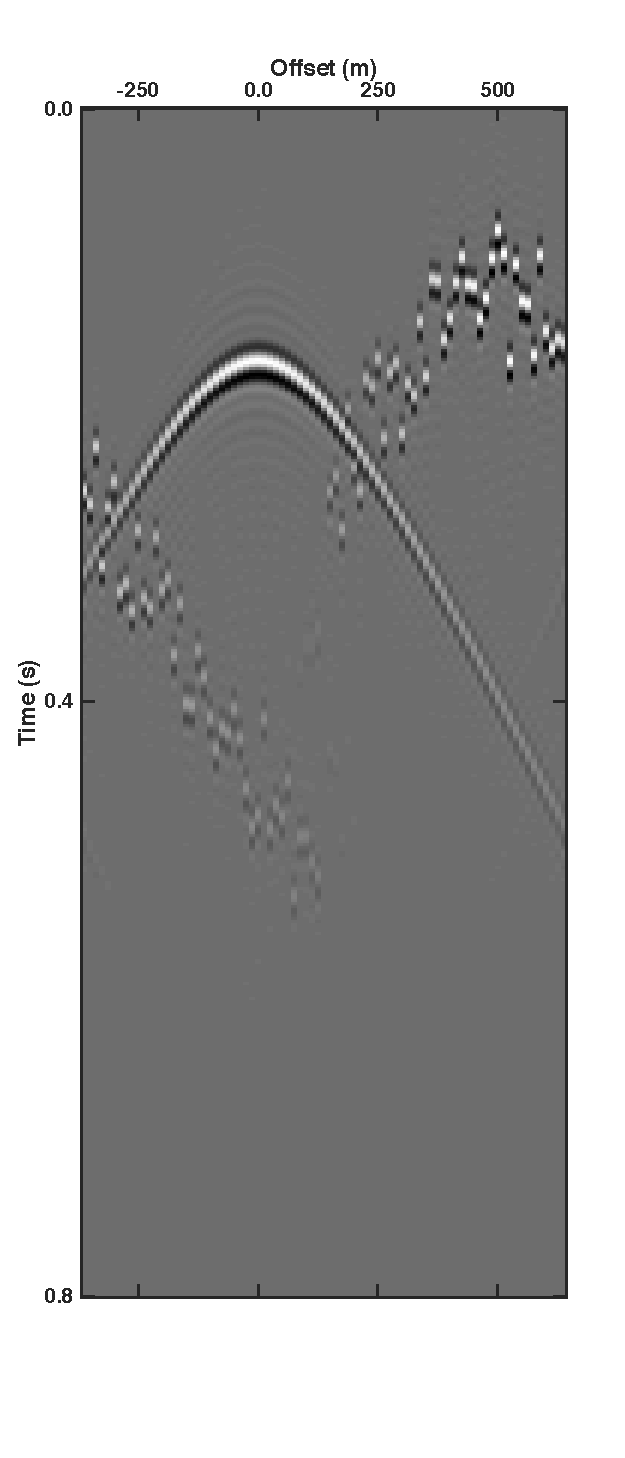
\includegraphics[width = \textwidth]{Plots/Mahdad/25iter/TimeDelay/Pseudo-DeblendedCRG_rec30}
		\caption{}
		\label{fig:Ch-Theory-PseudoCRG-IncoherentDelay}
	\end{subfigure}
	%
	\centering
	\begin{subfigure}[b]{0.3\textwidth}
	
		\centering
		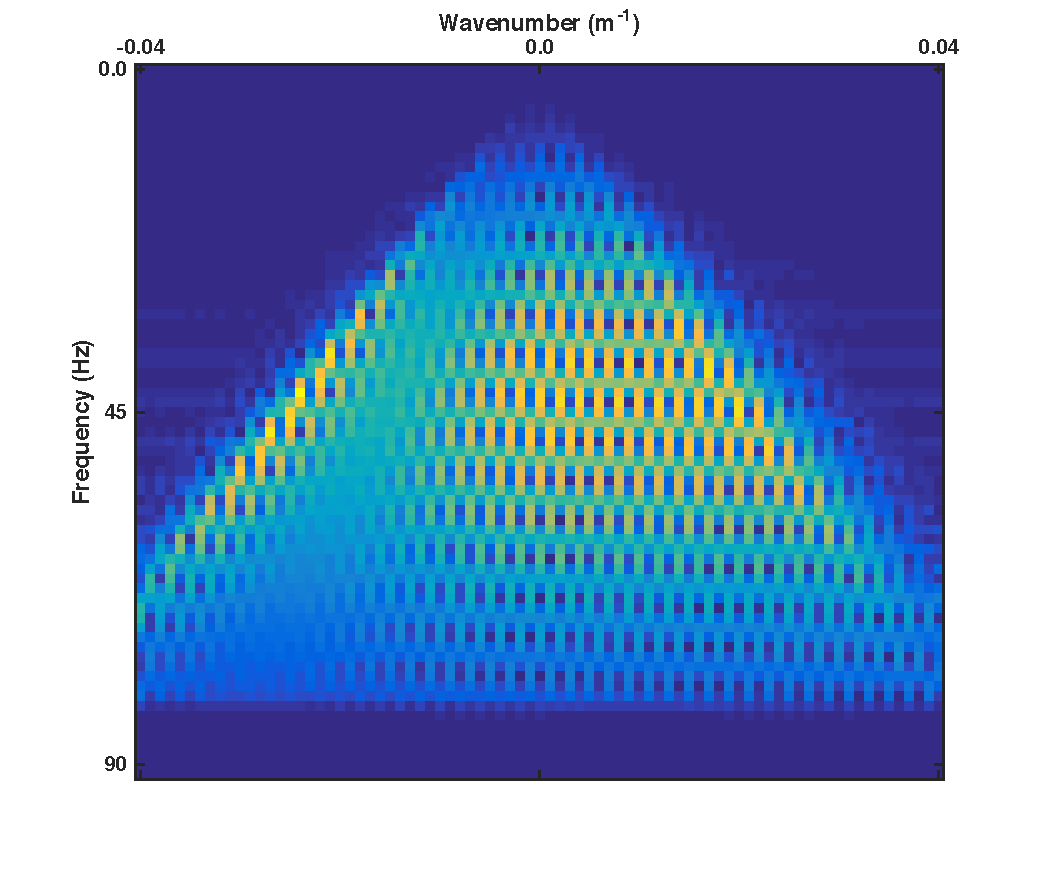
\includegraphics[width = \textwidth]{Plots/Mahdad/25iter/TimeDelay/FK-Pseudo-deblendedCRG_rec30_coh}
		\caption{}
		\label{fig:Ch-Theory-PseudoCRG-FK-CoherentDelay}
		
		\par\bigskip
		
		\centering
		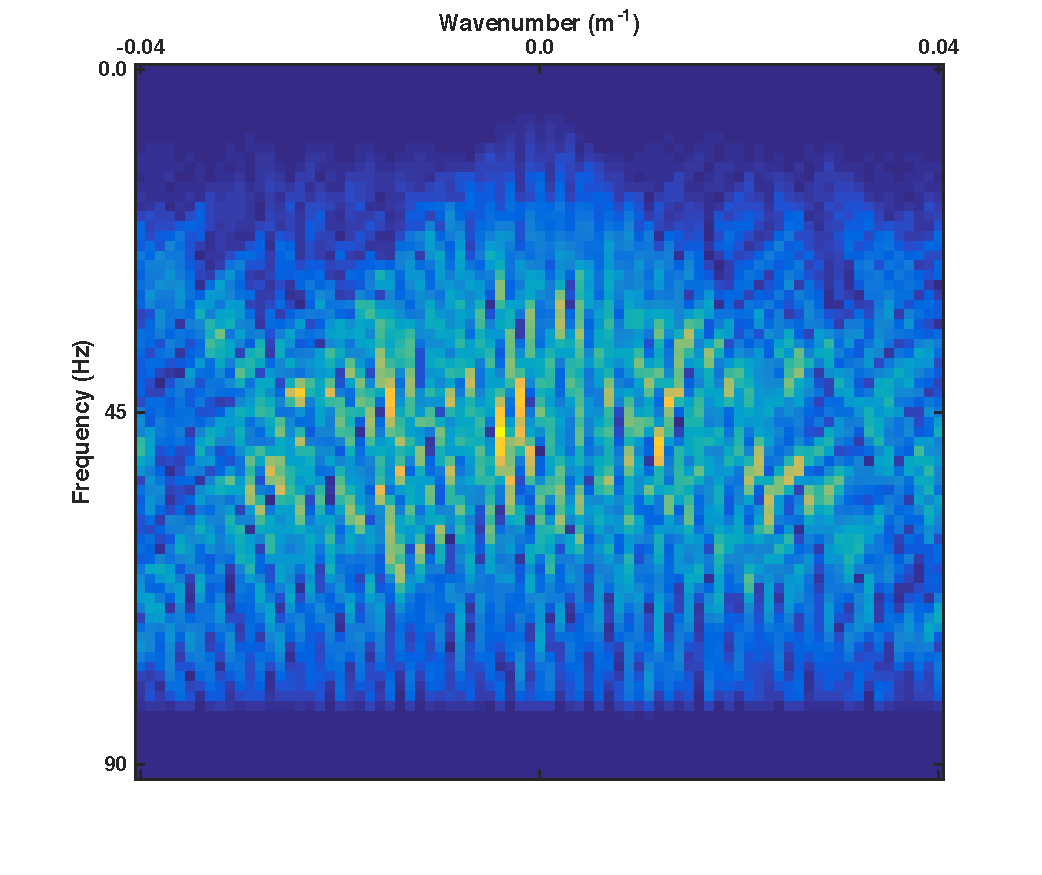
\includegraphics[width = \textwidth]{Plots/Mahdad/25iter/TimeDelay/FK-Pseudo-deblendedCRG_rec30}
		\caption{}
		\label{fig:Ch-Theory-PseudoCRG-FK-IncoherentDelay}
		
	\end{subfigure}
	
	\caption{Comparison of the pseudo-deblended receiver gather for (a) constant firing time delays of \SI{100}{\milli\second}, and (b) random firing time delays between \SI{0}{\milli\second} and \SI{100}{\milli\second}. (c) and (d) show the $f$-$k$-spectra of (a) and (b) respectively.}
	\label{fig:Ch-Theory-PseudoCRG-IncoherencyEffect}

\end{figure}

\begin{figure}
	\centering
	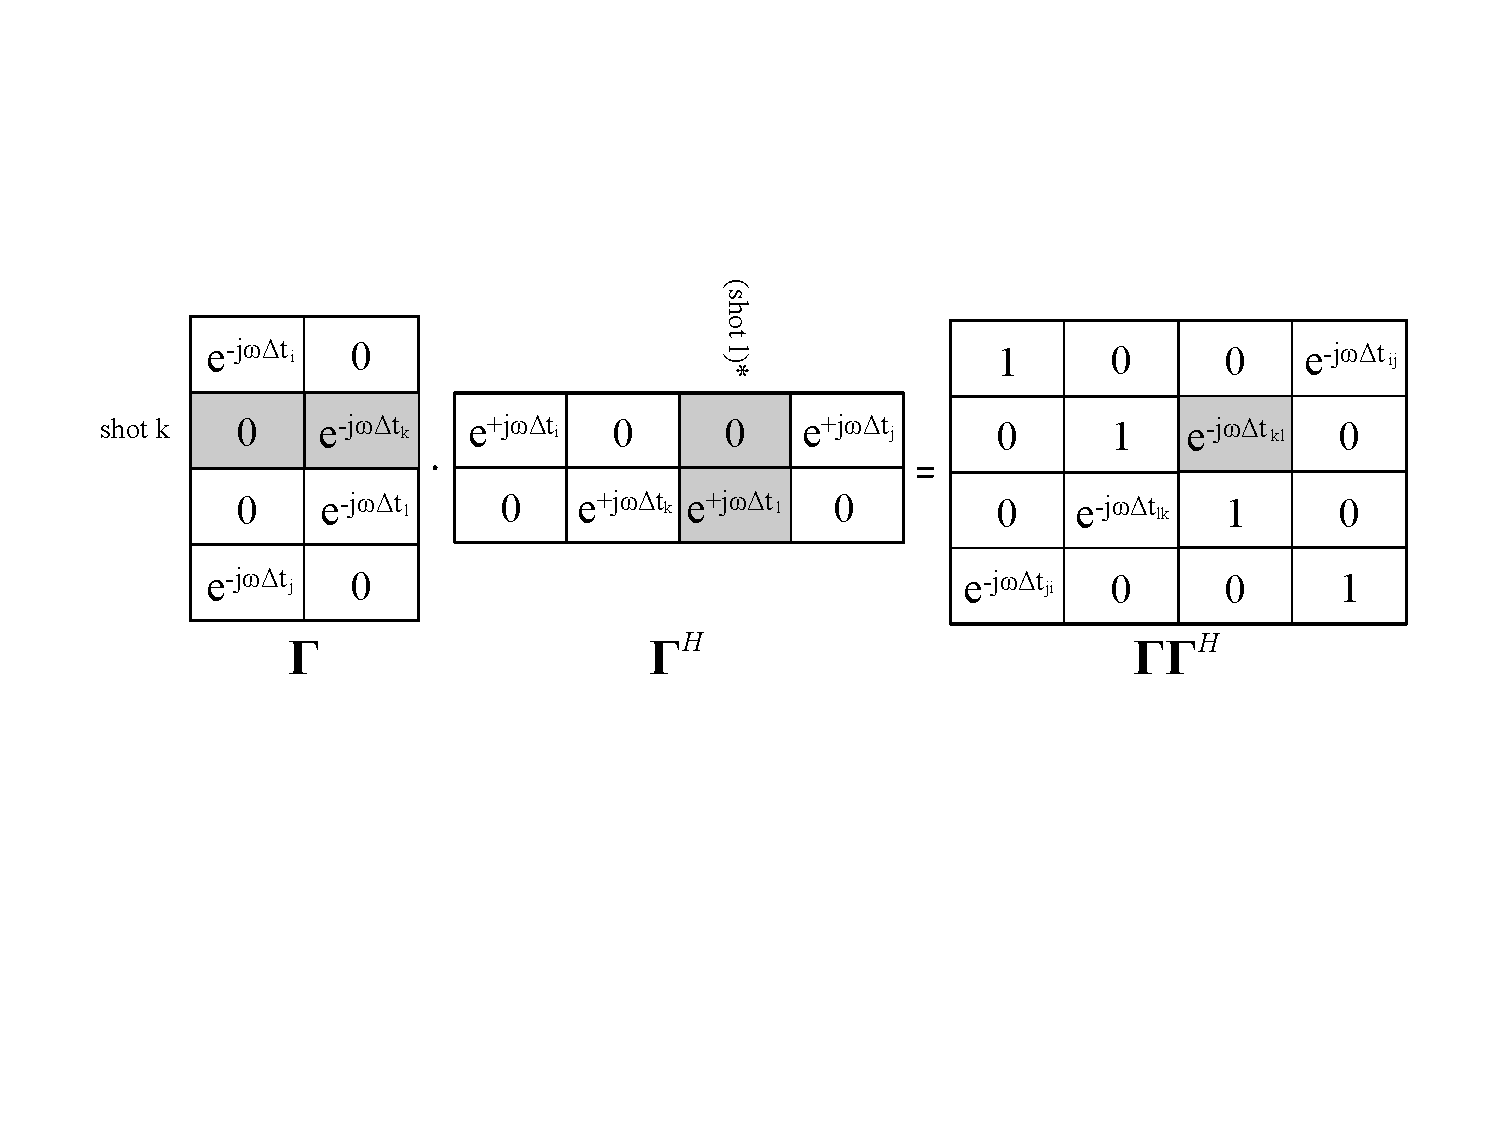
\includegraphics[width=\textwidth]{Plots/GGH_x}
	\caption{The blending matrix, $\mathbf{\Gamma}$, is obtained by interchanging the $3^{rd}$ and $4^{th}$ row of the blending matrix in Figure \ref{fig:Ch-Theory-GGH}. In acquisition this is equivalent to moving source 3 to experiment 2, and source 4 to experiment 1. A random permutation of the rows of the blending matrix spreads the off-diagonal elements of the matrix product, $\mathbf{\Gamma\Gamma}^H$. The elements are not assembled on the sub-diagonals anymore.}
	\label{fig:Ch-Theory-GGHx}
\end{figure}

\begin{comment}
In order to generate incoherent source interference, $\mathbf{N}$, it is therefore favorable if the elements $a_{ik}$ of each lower or upper diagonal are out of phase. For example, considering the $n^{th}$ upper or lower diagonal of the matrix $\mathbf{\Gamma \Gamma}^H$ this observation translates to the acquisition as follows: All source pairs, which are $n$ sources apart from each other, must be fired incoherently. The incoherent firing is realized by delaying blended sources with a random time delay.
\end{comment}

Of course, the degree of incoherency of the source interference, $\mathbf{N}$, also depends on whether the sources blended in an experiment are selected randomly, or in a spatially coherent pattern. For example, one expects the source interference to be more incoherent if in each experiment randomly picked sources are blended, than if in each experiment adjacent sources are blended (see Figure \ref{fig:Ch-Theory-GGHx}).

In 2D blending only adjacent sources can be blended, thus, the blended sources cannot be selected randomly. This changes when blending is extended to 3D: Within the crossline direction sources can be selected randomly and blended. 

\todo[inline]{This might need some extra explanation and plot!}

\begin{comment}

In terms of the blending matrix $\mathbf{\Gamma}$ a spatially incoherent firing pattern means that the rows, i.e. the sources, are shuffled randomly. As a consequence the off-diagonal elements of the matrix product $\mathbf{\Gamma \Gamma}^H$ are reordered randomly. This shuffling process can help to further distort the phase of the interfering sources. However, if the maximum allowed time delay between blended sources is aready large the spatially incoherent blending pattern will not increase the incoherency of the interfering sources.   

In practice, the maximum allowed firing time delay is limited by the available acquisition time. The spatial distribution of blended sources is constraint by the acquisition design.
	
\end{comment}


\FloatBarrier


		\chapter{Incoherency} \label{chap::incoherency}

When multiple sources are applied in one experiment the wavefields of the individual sources overlap. \cite{Mahdad-Deblending-Method} presented a method to separate the overlapping wavefields: A key step is pseudo-deblending, which yields the the desired unblended data superimposed by so called blending noise. This noise is generated by the overlap of the individual sources and can be removed with noise filters. However, if the individual wavefields overlap coherently, the blending noise will also be coherent and cannot be removed. In other words it is crucial to fire the sources incoherently.

In this chapter the incoherency of the source overlap is analyzed by considering three questions: Which factors control the incoherency? How can the incoherency be measured? How can the incoherency be maximized for an optimal deblending result?

\section{Incoherency Control Factors}

The deblended data can be represented by

\begin{equation}
	\mathbf{ P_{debl} } = \mathbf{X S \Gamma \Gamma ^H}.
	\label{eq:Ch-Incoherency-Deblended-Data}
\end{equation} 

Each of the matrices in the above equation influences the degree of incoherency of the source overlap. First, the contribution of the Earth \textbf{X} is neglected because it cannot be controlled in a seismic experiment. Second, the source signature \textbf{S}, in particular its time duration, determines the required minimum time delay between sources to avoid an overlap. Consequently, when designing an acquisition with simultaneous sources one must take into account the source signature. Thirdly, the incoherency is strongly dependent on the blending matrix $\mathbf{\Gamma}$ because it captures the firing pattern, i.e. it knows which sources are superimposed and the time delays between the sources in a given experiment. Therefore, the main focus of the incoherency analysis will be on the blending matrix $\mathbf{\Gamma}$.

\section{Quantification of Incoherency}

A mathematical tool to express incoherency is the autocorrelation function $R(\tau)$,

\begin{equation}
	R(\tau) = \int\limits_{\mathbb{R}} f^*(x) f(x + \tau) \, \text{d} x.
	\label{eq:Ch-Incoherency-Autocorrelation}
\end{equation}

For example, in a 1D case the autocorrelation of a fully incoherent function is a spike at zero lag. If a coherent or repetitive pattern is present in a function the autocorrelation will also have non zero amplitudes at other lags. 

For comparative purposes the incoherency of a function $f(x)$ should be quantified. It is suggested to measure incoherency $\mu$ as the ratio of the squared zero lag autocorrelation and the sum of the squared autocorrelation amplitudes,

\begin{equation}
	\mu = \frac{R(\tau = 0)^2}{\sum\limits_{\tau} R(\tau)^2}	.
	\label{eq:Ch-Incoherency-Incoherency}
\end{equation} 

This expression quantifies incoherency as a number between 0 and 1. A fully incoherent function $f(x)$ yields an autocorrelation which is a perfect spike. Thus, the ratio in equation \ref{eq:Ch-Incoherency-Incoherency} equals 1. For a perfectly coherent function $f(x)$ the ratio in equation \ref{eq:Ch-Incoherency-Incoherency} is nearly zero.

The incoherency strongly depends on the blending matrix $\mathbf{\Gamma}$ which is a 3D array. Before applying an autocorrelation the blending matrix $\mathbf{\Gamma}$ is transformed to time domain. The time domain blending matrix is denoted as $\mathbf{\gamma}$. It has the dimensions

\begin{equation}
	\text{dim}(\mathbf{\gamma}) = \text{Sources x Experiments x Time}.
	\label{eq:Ch-Incoherency-gamma}
\end{equation}

If a source $s_i$ is fired in an experiment $e_i$ at a time $t_i$ the element $(s_i,e_i,t_i)$ of $\mathbf{\gamma}$ is 1, else it is 0. If the source is not a perfect spike its amplitude can smear out across several time samples in the matrix $\mathbf{\gamma}$.

The incoherency of the blending matrix $\mathbf{\gamma}$ can be quantified by replacing the 1D autocorrelation in equation \ref{eq:Ch-Incoherency-Autocorrelation} and \ref{eq:Ch-Incoherency-Incoherency} with a 3D autocorrelation, which can be written as,

\begin{equation}
	R(\tau_1,\tau_2,\tau_3) = \iiint\limits_{\mathbb{R}^3} f^*(x,y,z) f(x + \tau_1,y + \tau_2, z + \tau_3) \, \text{d} x \, \text{d} y \, \text{d} z.
	\label{eq:Ch-Incoherency-3dAutocorrelation}
\end{equation}

\todo[inline]{The calculation of the 3D autocorrelation function requires significant computational power such that symmetry properties of the autocorrelation should be exploited to reduce the cost. Symmetry with respect to the origin, but using convn in Matlab I cannot access it}

The elements of the resulting 3D autocorrelation array are a measure for the correlation between wavefields at a specific source, experiment and time lag. For example, if in each experiment adjacent sources are fired with a constant time delay $\Delta t$, the 3D autocorrelation will yield a high amplitude at the source lag 1, experiment lag 0 and time lag $\Delta t$.

Combining equations \ref{eq:Ch-Incoherency-Incoherency} and \ref{eq:Ch-Incoherency-3dAutocorrelation} the incoherency of the time domain blending matrix $\mathbf{\gamma}$ can be expressed as,

\begin{equation}
	\mu = \frac{R(\tau_1 = 0,\tau_2 = 0,\tau_3 = 0)^2}{\sum\limits_{(\tau_1,\tau_2,\tau_3)} R(\tau_1,\tau_2,\tau_3)^2}	.
	\label{eq:Ch-Incoherency-Incoherency3d}
\end{equation} 

\section{Optimization of Incoherency}

\todo[inline]{Relate the incoherency estimate to the quality factor of the deblending. Point out that the quality factor is very sensitive to the time incoherency while the incoherency with respect to experiments or sources has less impact on the deblending performance.}

\section{Fingerprint of the Incoherency in the Blending Matrix $\mathbf{\Gamma}$}

To achieve a better understanding of the blending process the relation between the incoherency quantification and the blending matrix $\Gamma$ is assessed.

In frequency domain the blending matrix has the dimension,

\begin{equation}
	\text{dim}(\mathbf{\Gamma}) = \text{Sources x Experiments x Frequency},
	\label{eq:Ch-Incoherency-Dim-Gamma}
\end{equation}

where each element is a complex number $a \mathrm{e}^{ - \mathrm{j} \omega t }$.























\cite{Mahdad-Deblending-Method}

%
% Biblio
    \bibliographystyle{apalike}
    \printbib{my_bib} % in MyBib.bib you add all your reference information, following the correct format. Sometimes, the bib file needs to be built several times, as well as the main file, before all references occur correctly in your PDF. 


%============================= Back matter =========================================
\appendix

    \chapter{The back of the thesis}

    \section{An appendix section}

    \subsection{An appendix subsection with C++ Lisitng}

    \lstset{language=C++}
    \lstinputlisting{test.c}

    \subsection{A \matlab $ $ Listing}

    \lstset{language=matlab}
    \lstinputlisting{test.m}

    \chapter{Yet another appendix}

    \section{Another test section}

    Ok, all is well.

% Index
    \printindex%
    \cleardoublepage%

\end{document}

